\documentclass[]{beamer}
\usepackage{url}
\usepackage{tikz}
\usepackage{pgfplots}
\usepackage[framemethod=tikz]{mdframed}
\hypersetup{pdfstartview={Fit}} % Fit the presentation to the window when first displayed
\usetheme{Frankfurt}

% http://danielfalster.com/blog/2013/06/18/a-nice-title-page-for-beamer-presentations/
\newmdenv[tikzsetting={draw=black,fill=white,fill opacity=0.7, line width=1pt},backgroundcolor=none,leftmargin=0,rightmargin=0,innertopmargin=5pt,skipbelow=\baselineskip,skipabove=\baselineskip]{TitleBox}

\title{Decoding Weather Satellites}
\author[Swartz]{Tom~Swartz}
\institute{Central PA Open Source Conference 2018}
\date{December 2018}
\subject{Computer Science}
\begin{document}

% Title Page
{\usebackgroundtemplate{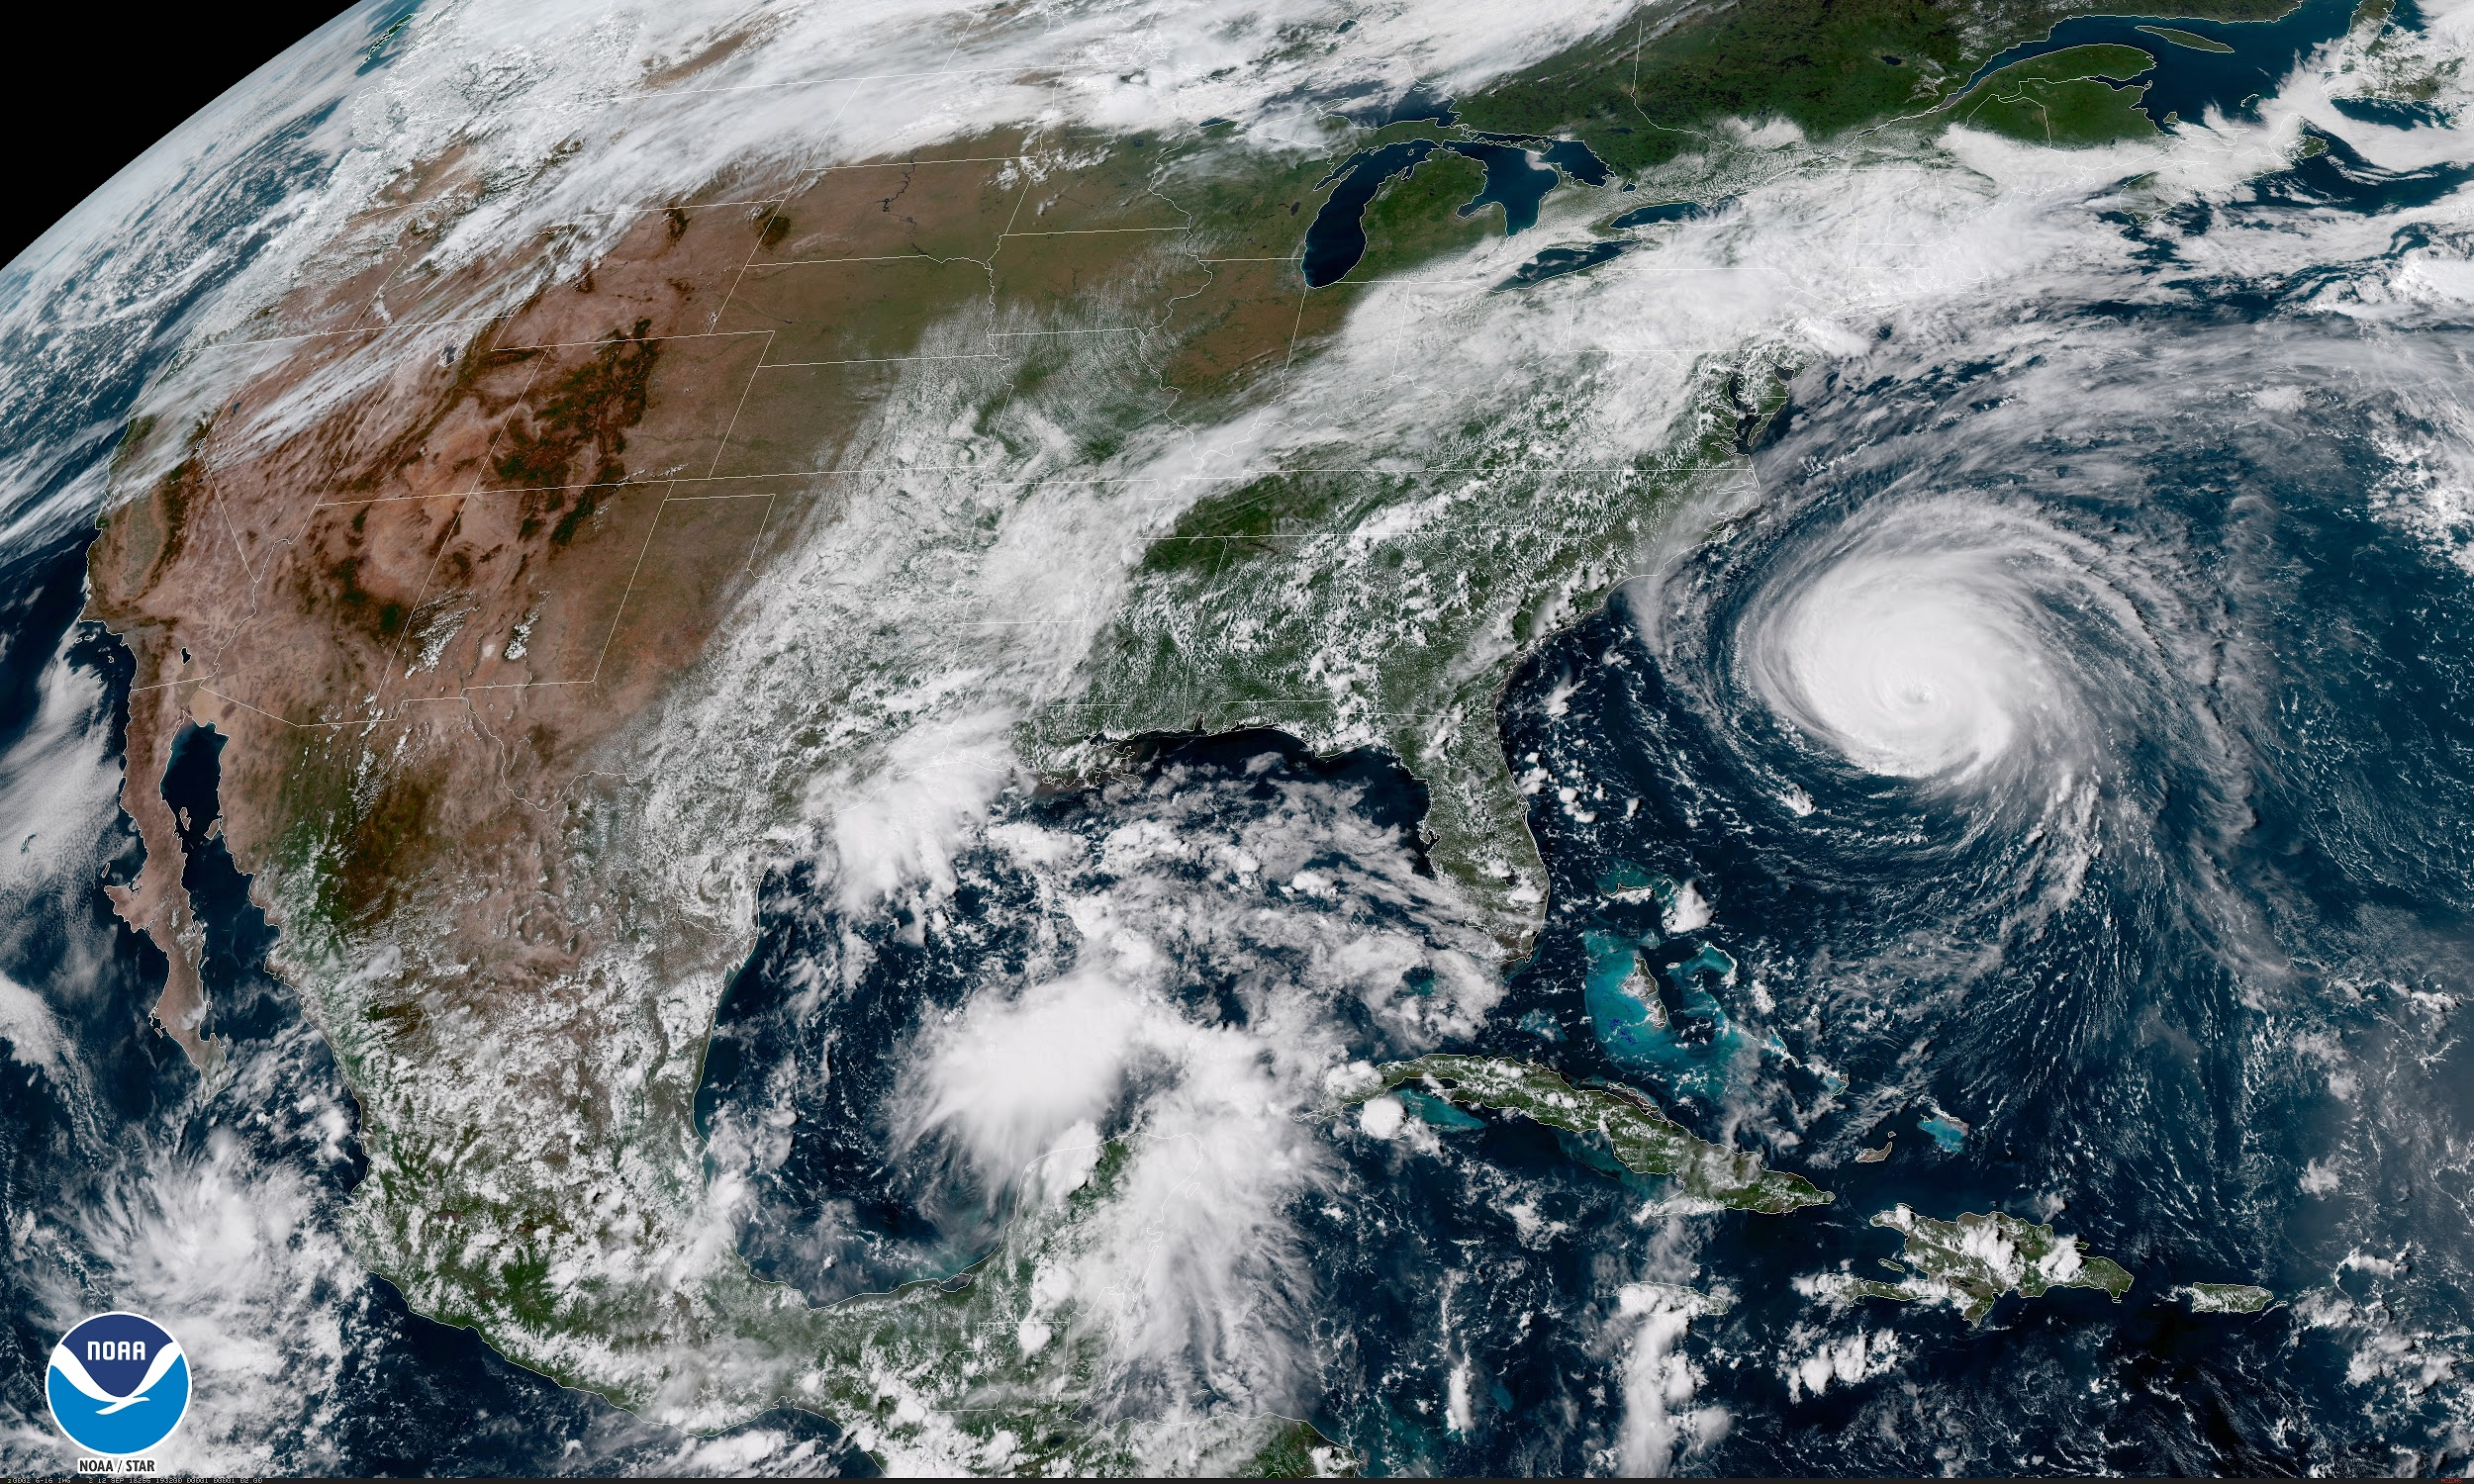
\includegraphics[height=1.0\paperheight,keepaspectratio]{images/goes.jpg}}
\begin{frame}[plain]
    \vspace{17em}
    \begin{TitleBox}
        \begin{center}
            {\color{red}\huge\inserttitle\color{black}}\\
        \end{center}
        \insertauthor{}\hfill\insertinstitute{}\\
        {\footnotesize
        \href{http://twitter.com/tswartz07}{@tswartz07}
        \hfill
        \href{mailto: tom@tswartz.net}{tom@tswartz.net}
        }
    \end{TitleBox}
\end{frame}}

\begin{frame}
    \frametitle{Who is this guy?}
    \framesubtitle{And what is he doing here?}
    \begin{columns}[T]
        \begin{column}[T]{5cm}
           {\huge Tom Swartz}
            \begin{itemize}%[<+->]
                \item<1->{Using SDR since 2012}
                \item<1->{Not my day job, just a hobby}
                \item<1->{Not affiliated with NOAA}
                \item<1->{Captured \textgreater120 satellite passes over 6 years}
                \item<1->{Involved in ham radio}
                \item<1->{Listened to lots of amateur radio}
                \item<2->{My dog's name is Wilbur}
            \end{itemize}
        \end{column}
        \begin{column}[T]{5cm}
            
\includegraphics[height=6cm]{images/me.jpg}
        \end{column}
    \end{columns}
\end{frame}

% What's ahead?
\begin{frame}
    \frametitle{Agenda}
    \tableofcontents
\end{frame}

% Lets get into it now...

\section[Background]{Background of Weather Satellites}
\begin{frame}
    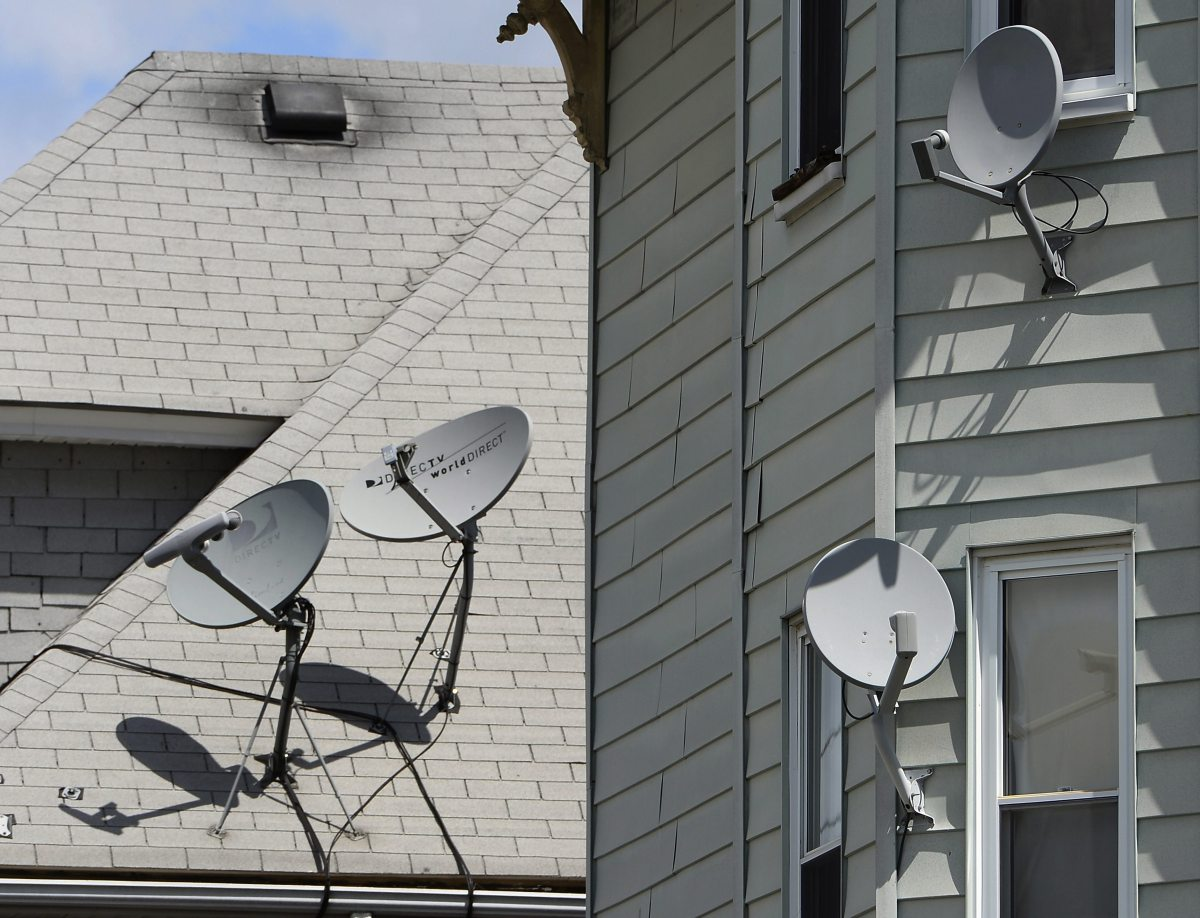
\includegraphics[]{images/dish.jpg}
\end{frame}

\subsection{NOAA POES}
\begin{frame}
    \frametitle{Polar-orbiting Operational Environmental Satellite 19}
    \framesubtitle{Launched: 6 Feb 2009}
    \begin{columns}[T]
        \begin{column}[T]{5.5cm}
            \begin{itemize}
                \item 535 Miles
                \item Lancaster $\to$ Charleston,~SC
                \item 2.9 ms for light to travel
                \item Camera resolution: 2.5~Miles/Pixel
            \end{itemize}
            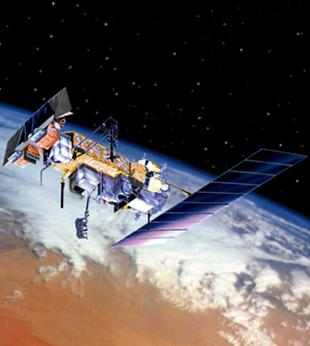
\includegraphics[height=4cm,keepaspectratio]{images/noaa-19-sat-illus.png}
        \end{column}
        \begin{column}[T]{5cm}
            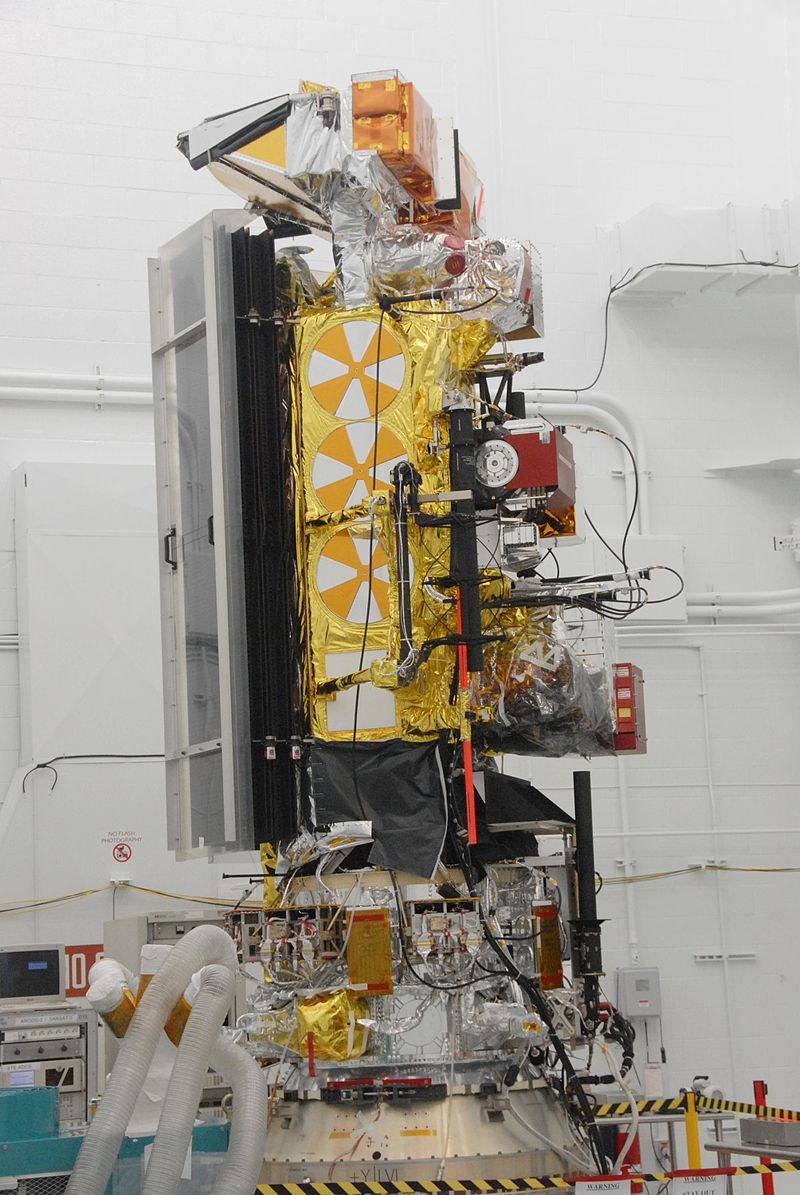
\includegraphics[height=7cm]{images/noaa19-sat.jpg}
        \end{column}
    \end{columns}
\end{frame}
\subsection{Meteor M2}
\begin{frame}
    \frametitle{Roscosmos Meteor 3M-2}
    \framesubtitle{Launched: 8 July 2014}
    \begin{columns}[T]
        \begin{column}[T]{5.5cm}
            \begin{itemize}
                \item 515 Miles
                \item Lancaster $\to$ Louisville,~KY
                \item 2.8 ms for light to travel
                \item Camera resolution: 1.8~Miles/Pixel
            \end{itemize}
        \end{column}
        \begin{column}[T]{5cm}
            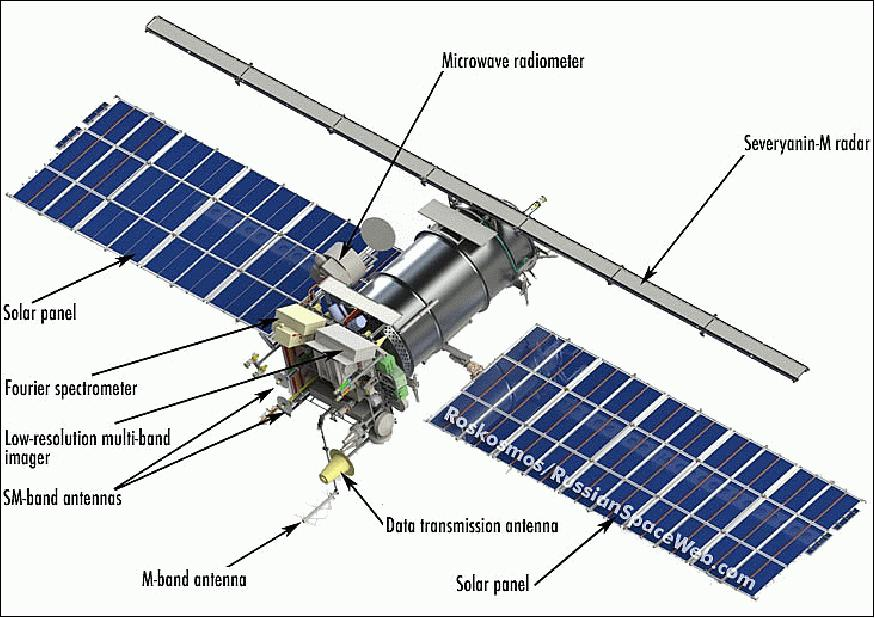
\includegraphics[height=4cm,keepaspectratio]{images/meteor-m2.jpg}
        \end{column}
    \end{columns}
\end{frame}
\subsection{NOAA GOES}
\begin{frame}
    \frametitle{Geostationary Operational Environmental Satellite-16}
    \framesubtitle{Launched: 19 Nov 2016}
    \begin{columns}[T]
        \begin{column}[T]{6.1cm}
            \begin{itemize}
                \item 22,236 Miles
                \item Lancaster $\to$ Venezuela (the long way)
                \item 119 ms for light to travel
                \item Camera resolution: 0.35~Miles/pixel~(1900~feet/pixel)
            \end{itemize}
            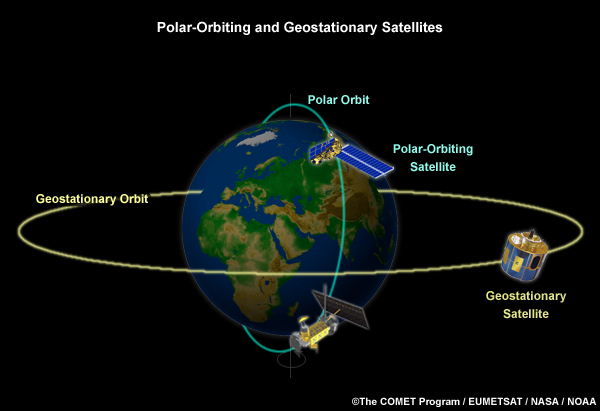
\includegraphics[height=4cm,keepaspectratio]{images/polar-vs-geo-satellites.jpg}
        \end{column}
        \begin{column}[T]{4cm}
            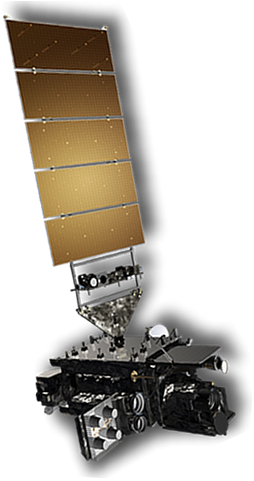
\includegraphics[height=6cm,keepaspectratio]{images/goes-r-illus.png}
        \end{column}
    \end{columns}
\end{frame}


\section{Introduction to SDR}
\subsection{Crash Course in SDR}
\begin{frame}
    \frametitle{Software Defined Radio}
    \framesubtitle{Crash Course in SDR}
    \begin{center}
        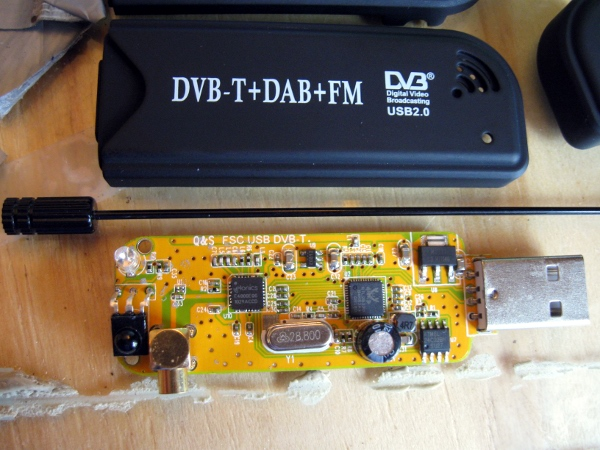
\includegraphics[width=0.75\paperwidth,height=1.0\paperheight,keepaspectratio]{images/rtlsdr.jpg}
    \end{center}
\end{frame}
\begin{frame}
    \frametitle{Software Defined Radio}
    \framesubtitle{SDR Hardware}
    \begin{columns}[T]
        \begin{column}[T]{5cm}
            \begin{itemize}
                \item{Very inexpensive radio}
                \item{Can receive 24~MHz to 2~GHz}
                \item{Uses computer software to interpret signals, rather than discrete transistors and expensive radio hardware}
            \end{itemize}
        \end{column}
        \begin{column}[T]{5cm}
            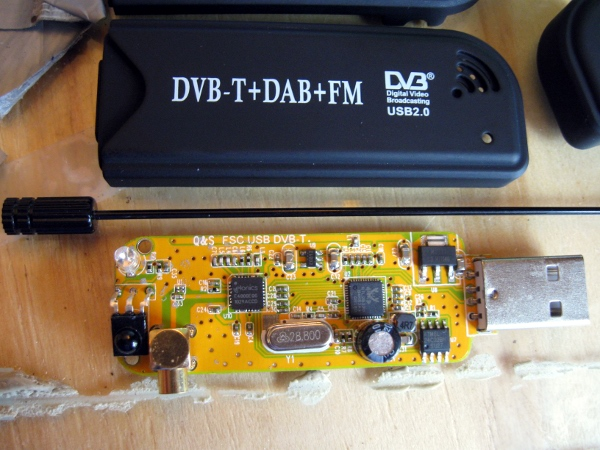
\includegraphics[height=4cm]{images/rtlsdr.jpg}
        \end{column}
    \end{columns}
\end{frame}
\begin{frame}[fragile]
    \frametitle{Frequencies}
    % https://tex.stackexchange.com/questions/98695/how-do-i-generate-a-logarithmic-x-axis-without-a-y-axis
    \begin{center}
        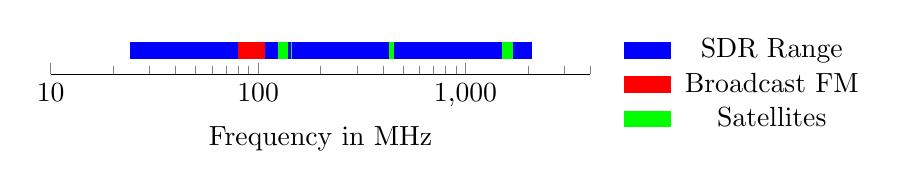
\begin{tikzpicture}
            \begin{axis}[
                    y=1.5cm,            % y unit vector
                    hide y axis,        % hide the y axis
                    legend style={draw=none},
                    legend pos=outer north east,
                    xmode = log,        % logarithmic x axis
                    axis x line*=bottom,% only show the bottom x axis line, without an arrow tip
                    log ticks with fixed point, % show layman numbers, not exponential format
                    xmin=10, xmax=4000,% range for the x axis
                    xlabel = Frequency in MHz
                ]
                \addplot [blue, no markers, line width=6pt] table {
                    24   1
                    2100 1

                };
                \addplot [red, line width=6pt] table {
                    80 1
                    108 1
                };
                \addplot [green, line width=6pt] table {
                    125 1
                    140 1
                };
                \addplot [green, line width=6pt] table {
                    144 1
                    146 1
                };
                \addplot [green, line width=6pt] table {
                    430 1
                    450 1
                };
                \addplot [green, line width=6pt] table {
                    1500 1
                    1700 1
                };
                \legend{SDR Range, Broadcast FM, Satellites}
            \end{axis}
        \end{tikzpicture}
        \begin{description}
            \item[RTL-SDR Range] 24~MHz $\to$ 2.1~GHz
            \item[Broadcast FM] 88~MHz $\to$ 108~MHz
            \item[Satellites] 130~MHz, 440~MHz, 1.9~GHz
        \end{description}
    \end{center}
\end{frame}
\begin{frame}
    \frametitle{Software Defined Radio}
    \framesubtitle{What types of things can SDR's receive?}
    \begin{itemize}
        \item Morse Code
        \item AM Radio
        \item Broadcast FM Radio
        \item IoT Devices
        \item Tire Pressure Monitoring Sensors
        \item Amateur Radio
        \item Ship Tracking
        \item Aircraft Tracking
        \item Baby Monitors
        \item Weather Balloons
        \item GPS Signals
        \item GSM Cell Phone Signals
        \item Taxi Dispatch
        \item Mall Security
        \item Remote Temperature Sensors
        \item \dots lots more
    \end{itemize}
\end{frame}
\subsection{Using SDR for Satellites}
\begin{frame}
    \frametitle{Software Defined Radio}
    \framesubtitle{Using SDR for Satellites}
    You need a few things:
    \begin{enumerate}
        \item A way to track the satellite
        \item An antenna to receive the satellite
            \begin{itemize}
                \item Omnidirectional antenna
                \item Dish antenna with motor mounts
                \item Plain dipole of appropriate size
            \end{itemize}
        \item A program to receive/record the signal
        \item A program to post-process and decode the signal
    \end{enumerate}
\end{frame}
\begin{frame}
    \frametitle{Software Defined Radio}
    \framesubtitle{Open Source Software for Satellites}
    \begin{enumerate}
        \item A way to track the satellite
            \begin{itemize}
                \item GPredict
                \item Predict
            \end{itemize}
        \item A program to receive/record the signal
            \begin{itemize}
                \item GQRX
                \item rtl\_fm
                \item rtl\_tcp
            \end{itemize}
        \item A program to post-process and decode the signal
            \begin{itemize}
                \item WXtoIMG
                \item MeDet
                \item MeteorDemod
                \item goestools
            \end{itemize}
    \end{enumerate}
\end{frame}



\section[Reception]{Receiving Satellite Signals}
\frame{\sectionpage}
\begin{frame}
    \frametitle{Tracking the Satellite}
    \begin{center}
        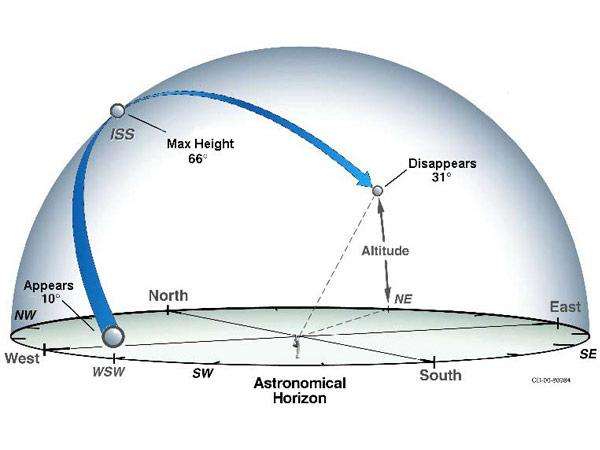
\includegraphics[width=0.75\paperwidth,height=1.0\paperheight,keepaspectratio]{images/az-el-vis.png}
    \end{center}
\end{frame}
\subsection{Receiving NOAA APT}
\begin{frame}
    There are currently three NOAA POES satellites working:
    \begin{description}
        \item[NOAA 15] \dotfill 137.620 MHz
        \item[NOAA 18] \dotfill 137.912 MHz
        \item[NOAA 19] \dotfill 137.100 MHz
    \end{description}
\end{frame}
\begin{frame}
    \frametitle{APT Signal}
    \begin{center}
        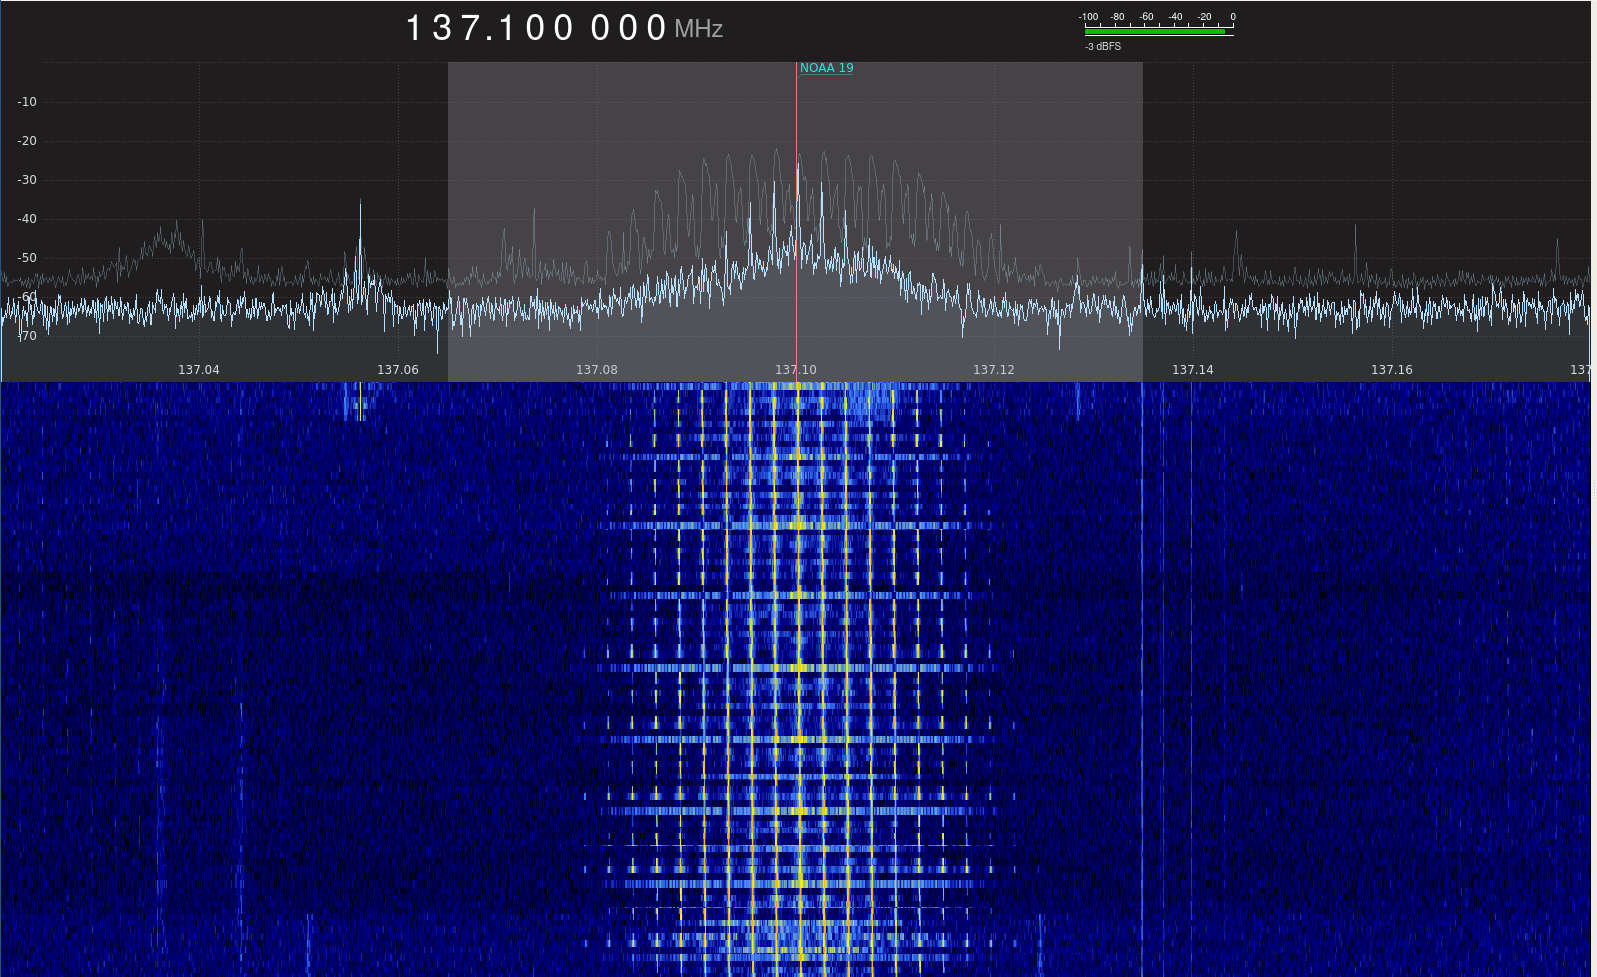
\includegraphics[width=0.75\paperwidth,height=0.75\paperheight,keepaspectratio]{images/apt-gqrx.png}
    \end{center}
\end{frame}
\subsection{Receiving METEOR LRPT}
\begin{frame}
    HRPT on POES, difficult to receive because of tracking
    HRPT on GOES, difficult because it's far away
\end{frame}
\subsection{Reception Problems?}
\begin{frame}
    \frametitle{Sometimes they break\dots}
    \framesubtitle{NOAA 15 System Status}
    \begin{center}
        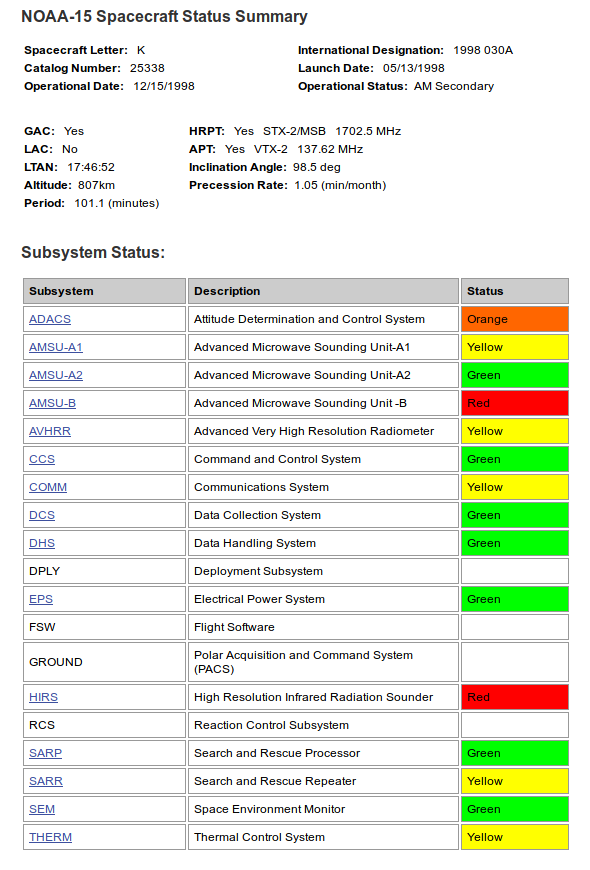
\includegraphics[width=0.75\paperwidth,height=0.75\paperheight,keepaspectratio]{images/noaa-15-status.png}
    \end{center}
\end{frame}
\begin{frame}
    \frametitle{Sometimes they break\dots}
    \framesubtitle{Meteor M2 Spinning}
    \begin{center}
        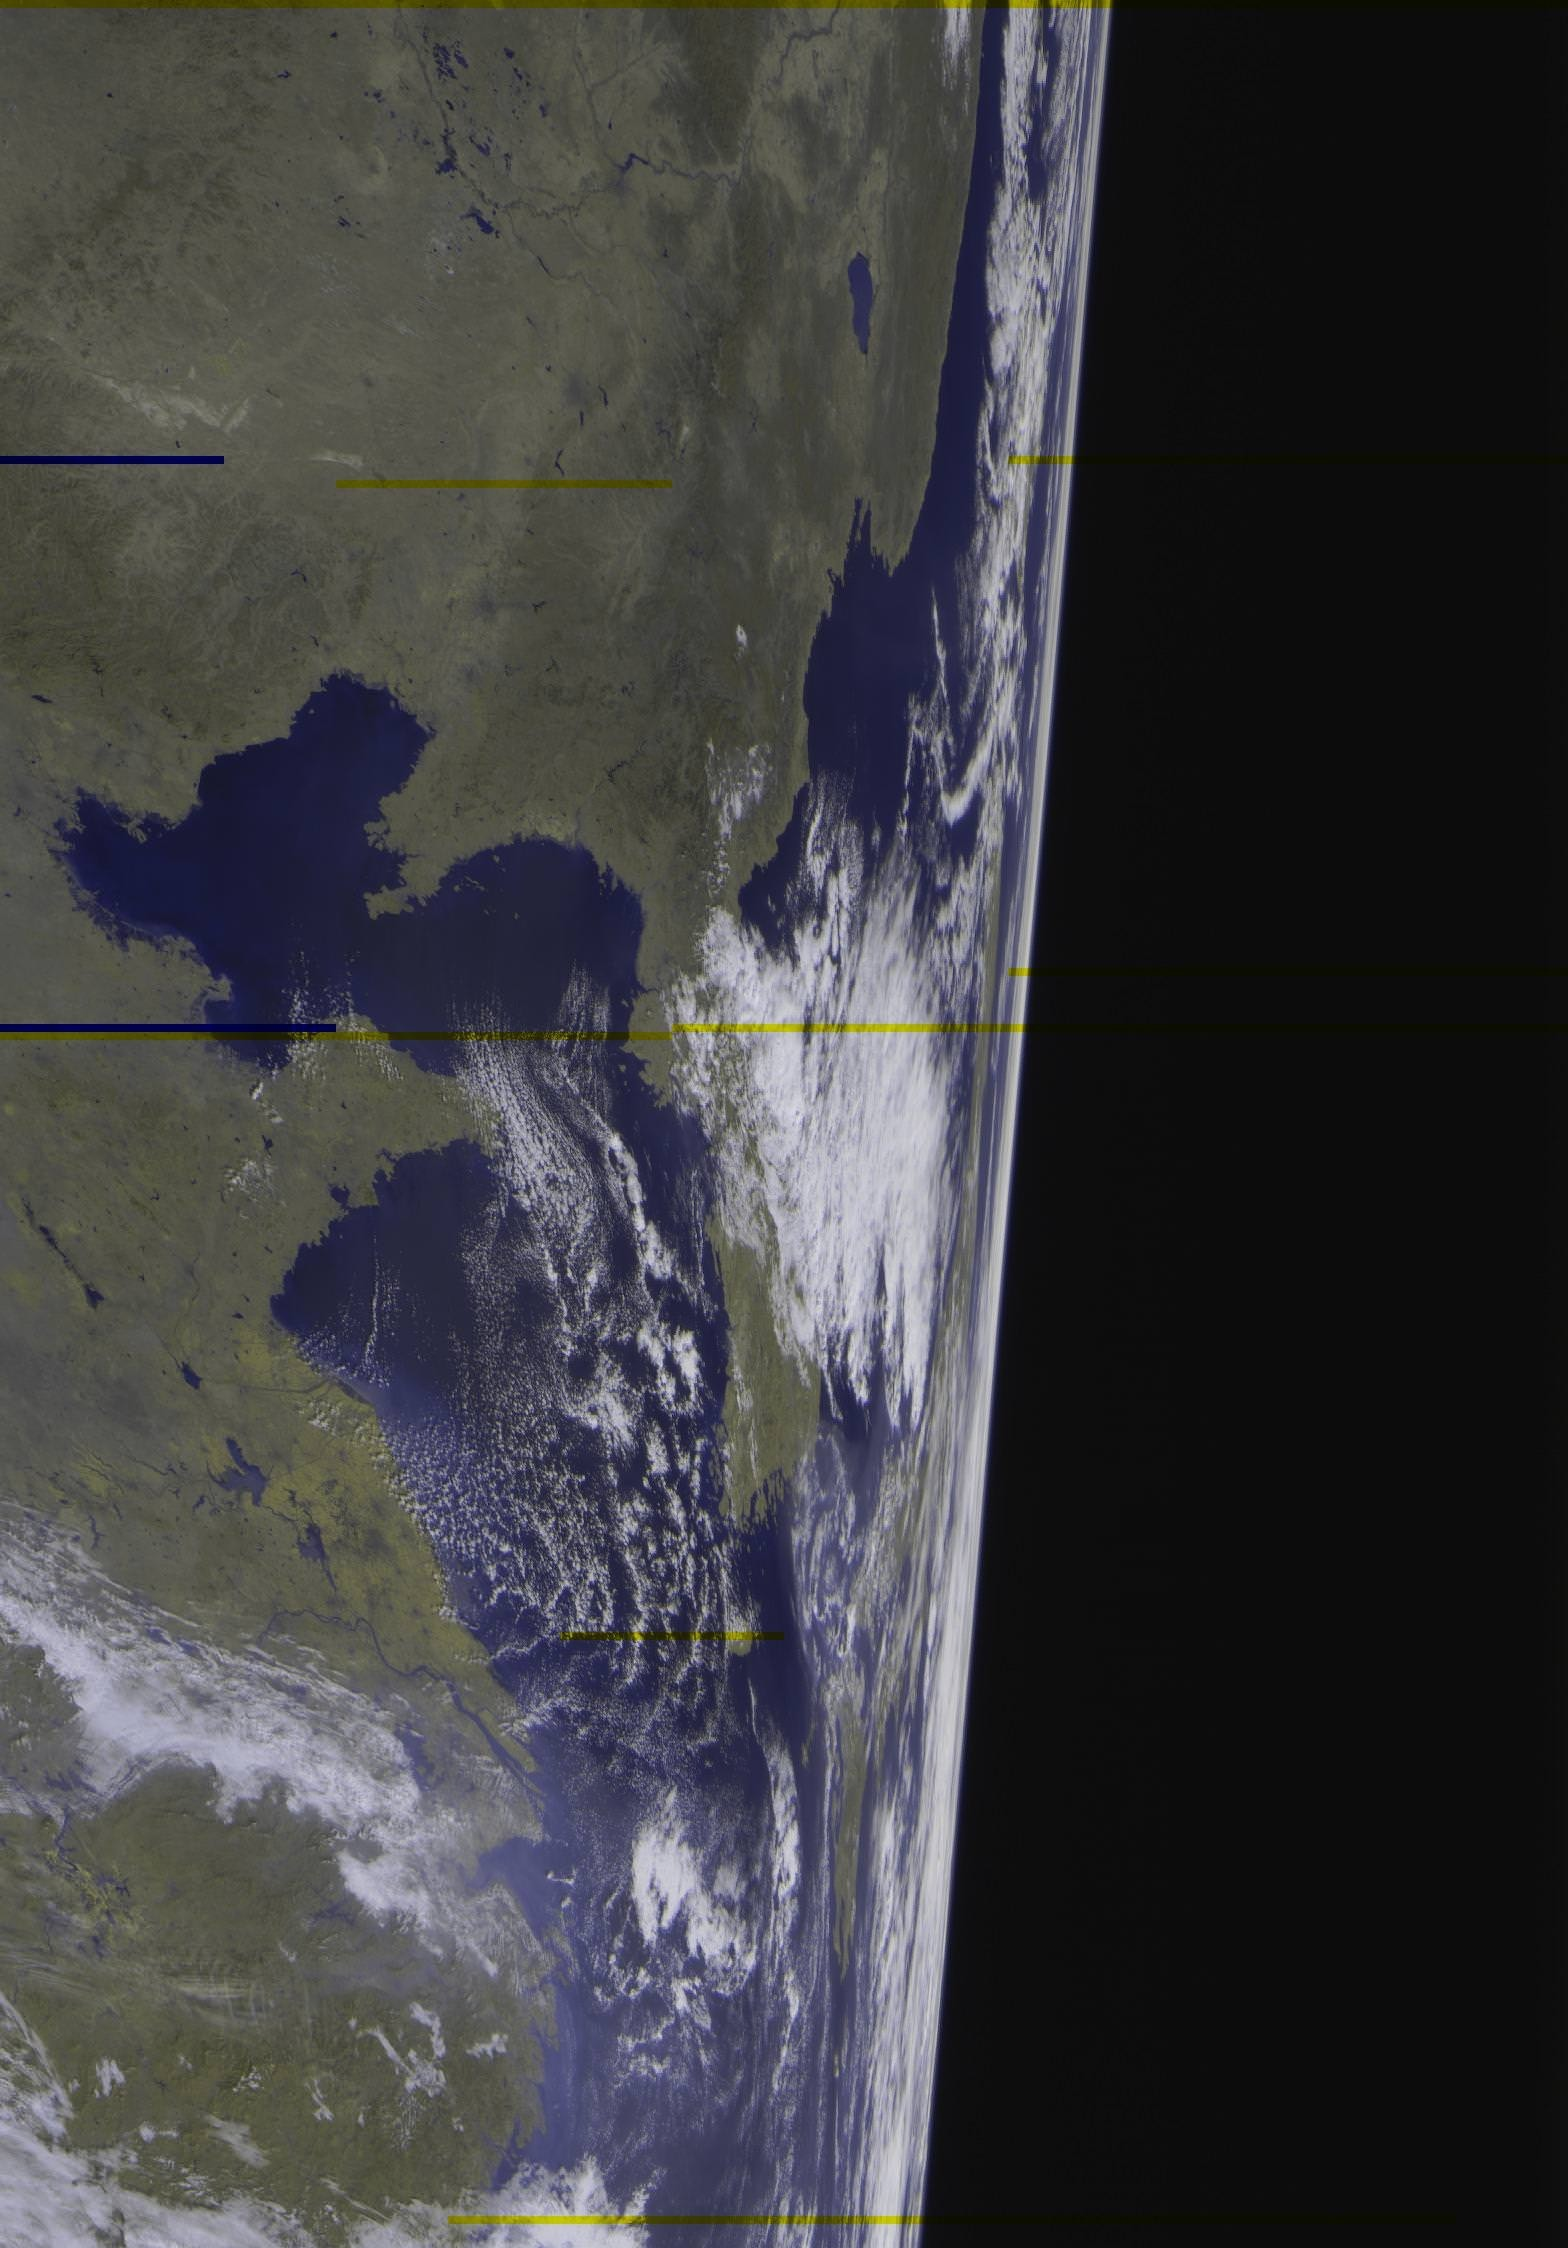
\includegraphics[width=0.75\paperwidth,height=0.75\paperheight,keepaspectratio]{images/meteor-spin.jpg}
    \end{center}
\end{frame}



\section[Decoding]{Decoding Satellite Signals}
\frame{\sectionpage}
\begin{frame}
    \frametitle{How do you get colors?}
    \framesubtitle{It's more complicated than you think!}
    \begin{center}
        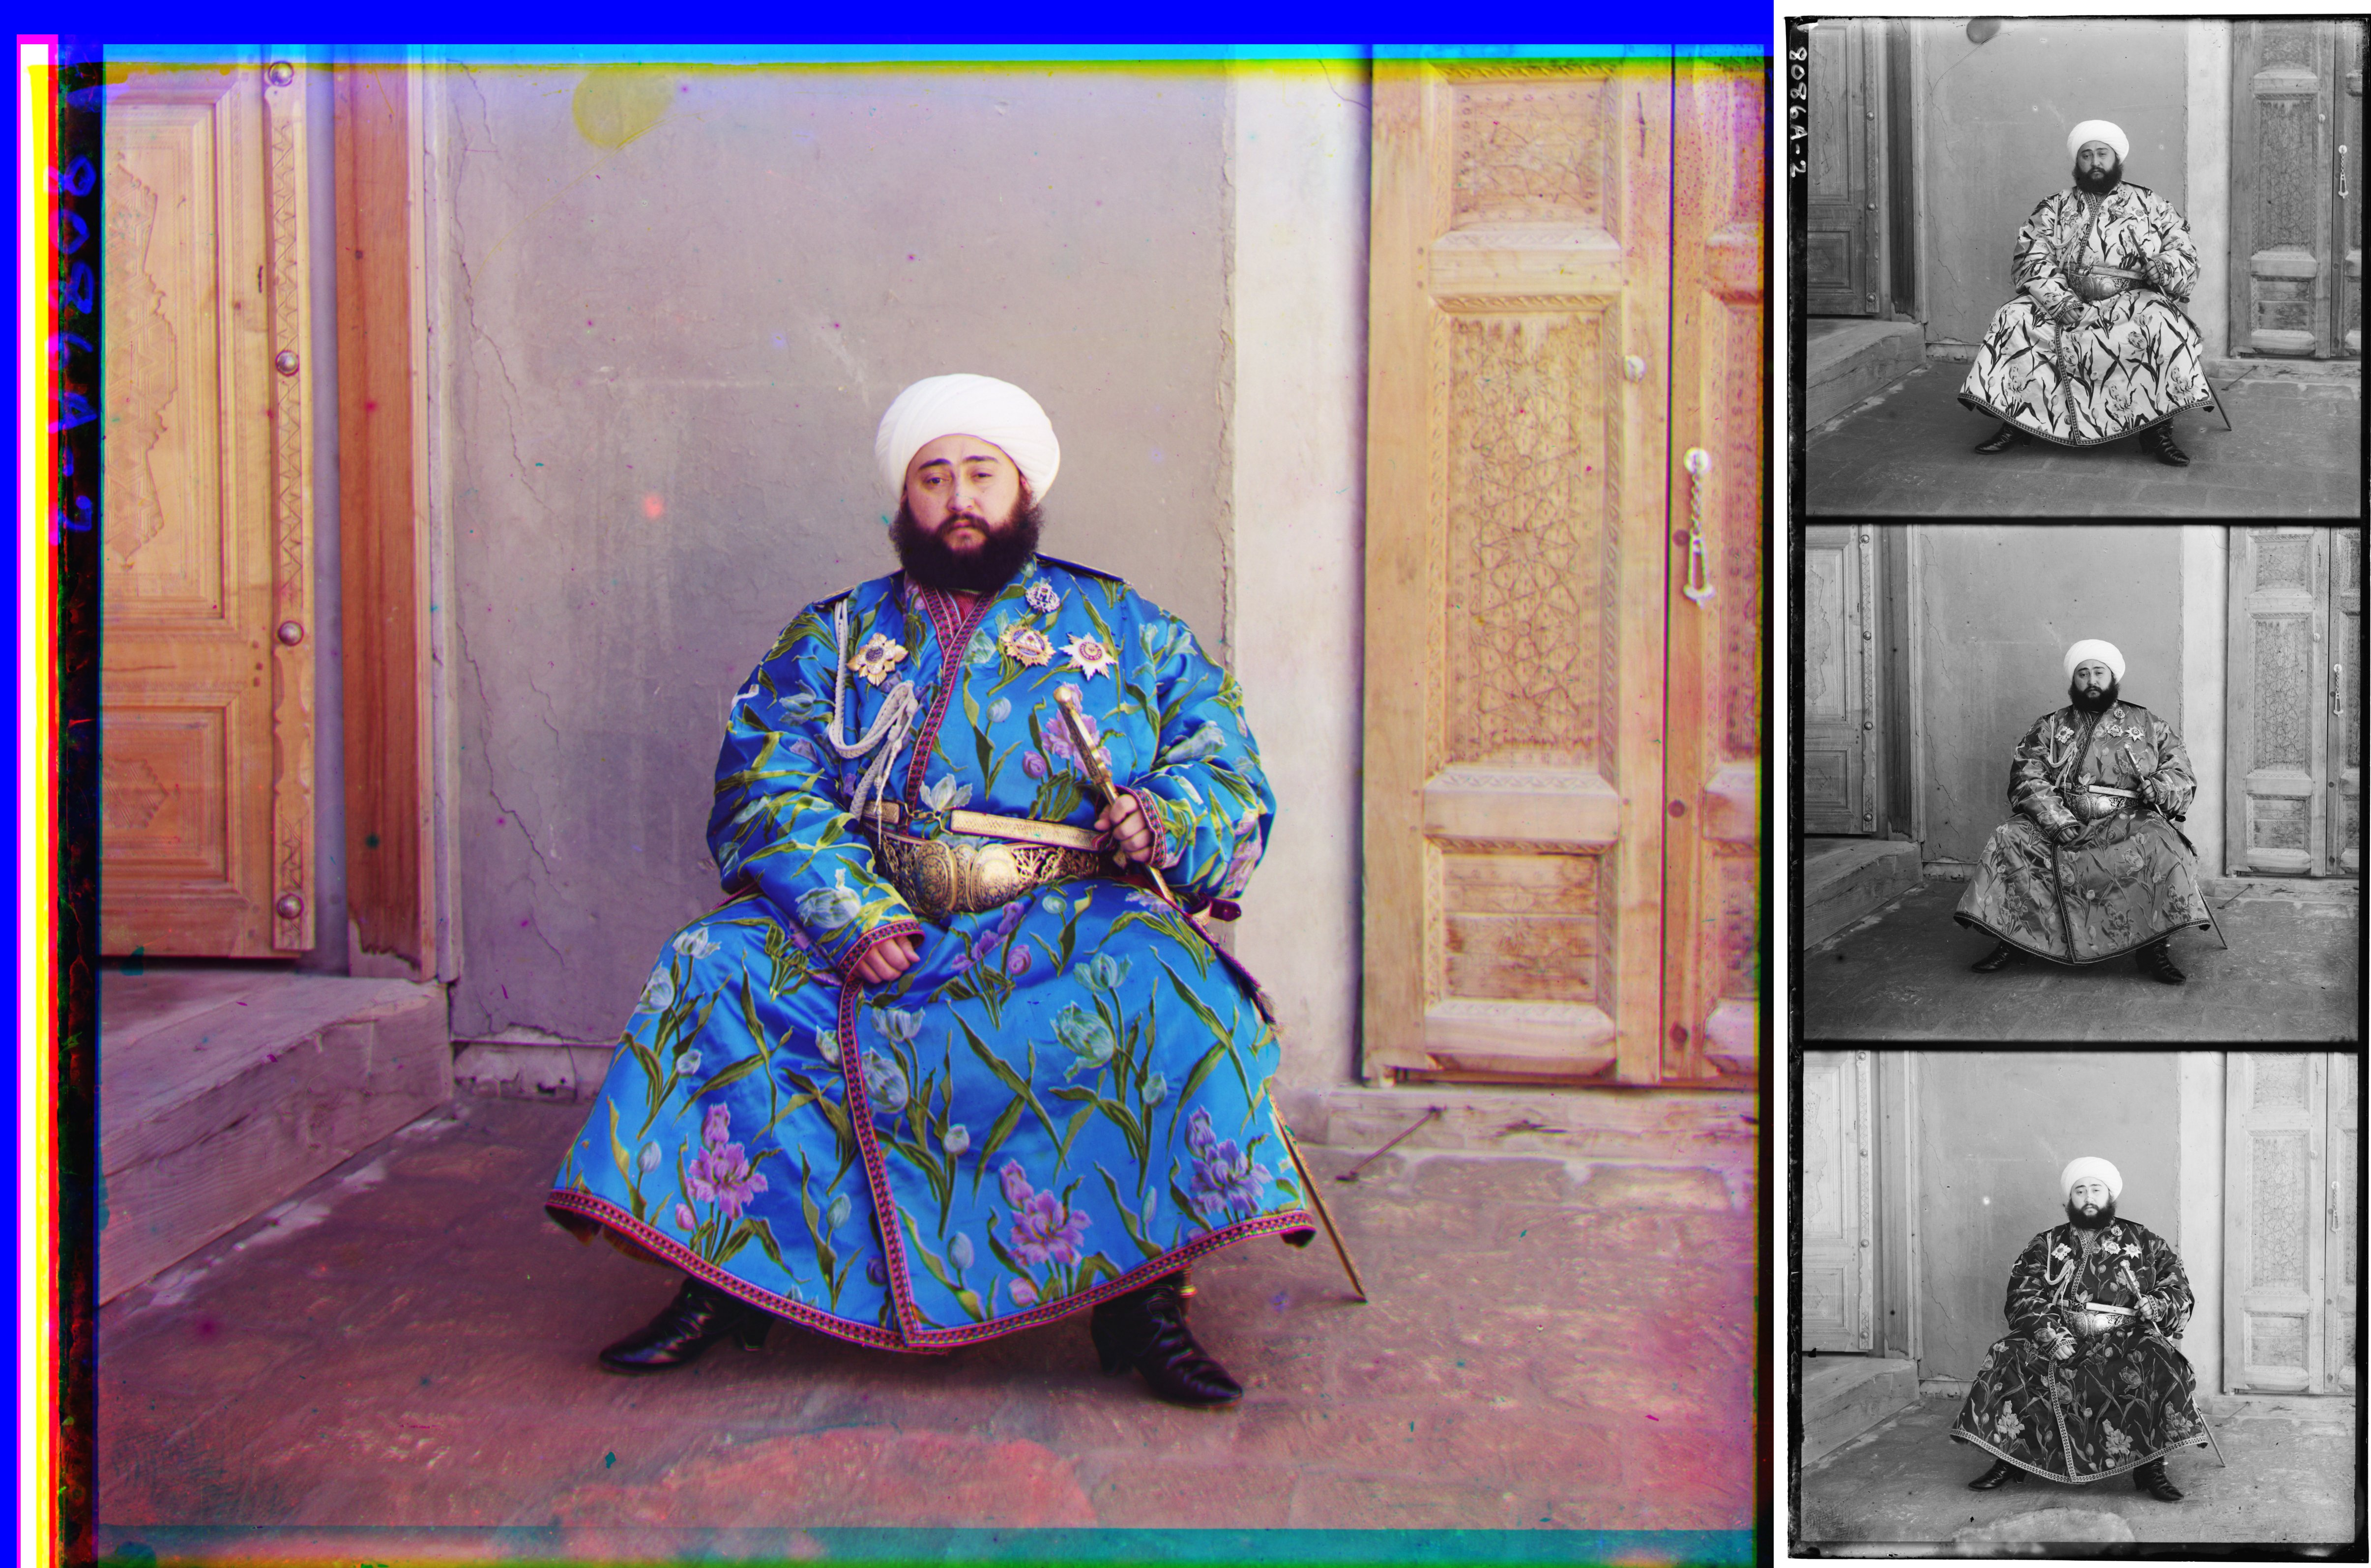
\includegraphics[width=0.80\paperwidth]{images/rgb-compose.jpg}
    \end{center}
\end{frame}
\subsection{Decoding NOAA POES APT}
\begin{frame}
    \frametitle{NOAA APT}
    \begin{columns}[T]
        \begin{column}[T]{5cm}
            \begin{itemize}
                \item First used in 1963
                \item Analog signal
                \item 2 Lines per Second (4160 Baud)
                \item 2080 Pixels wide, variable height
                \item Telemetry and picture data all in same line
            \end{itemize}
        \end{column}
        \begin{column}[T]{5cm}
            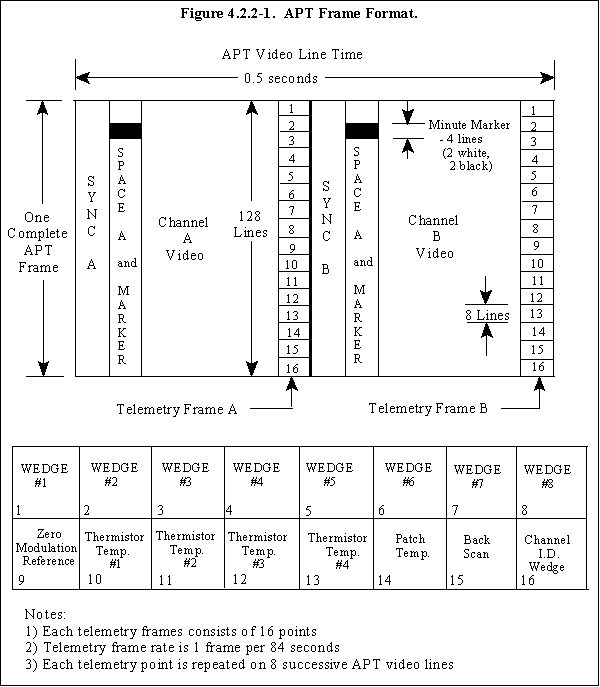
\includegraphics[height=0.5\paperwidth]{images/NOAA_APT_Frame_Format.png}
        \end{column}
    \end{columns}
\end{frame}
\begin{frame}
    \frametitle{NOAA APT}
    \begin{columns}[T]
        \begin{column}[T]{5cm}
            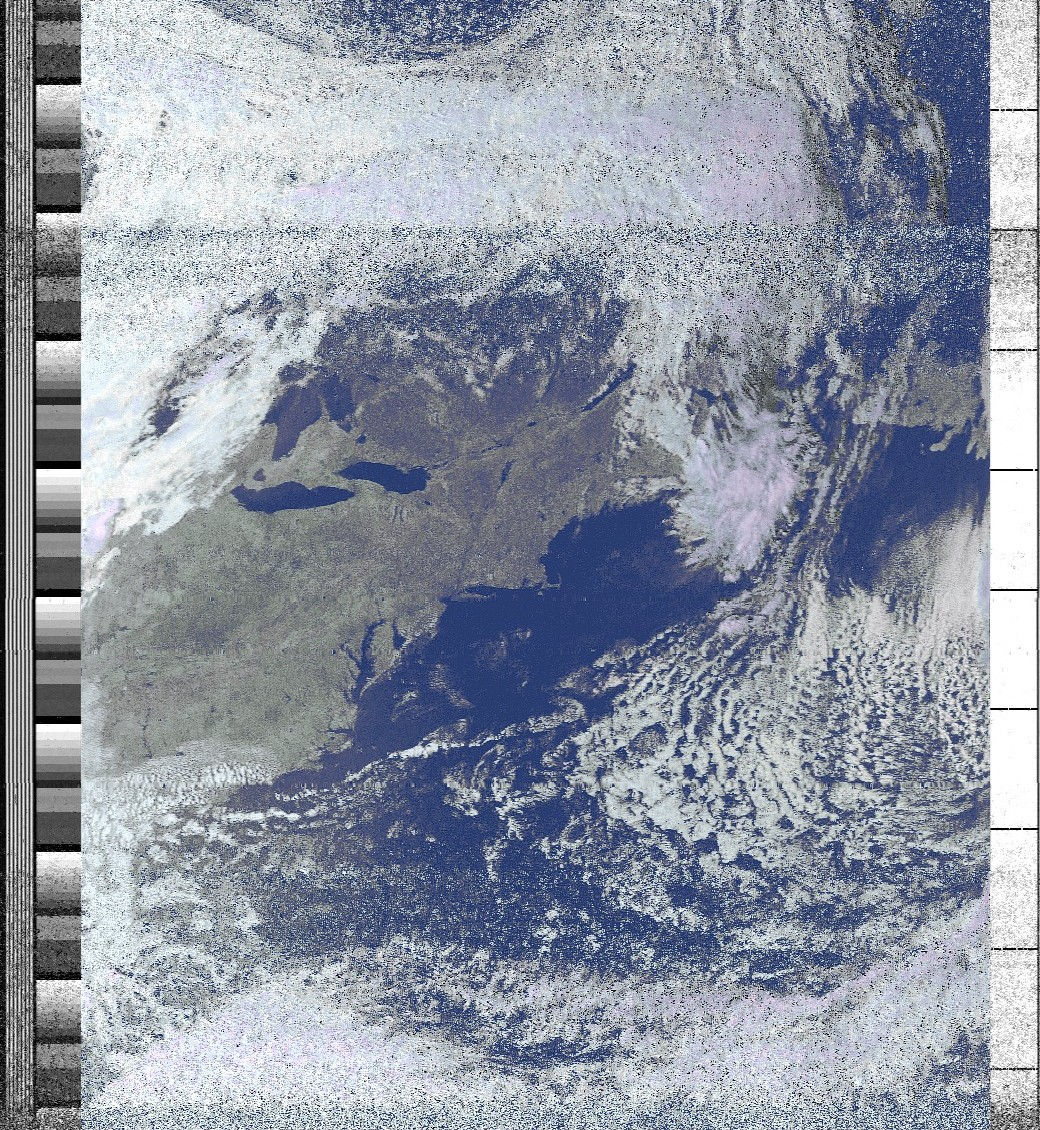
\includegraphics[height=0.5\paperwidth]{images/noaa-19-03-10-2017-1941-hvct.jpg}
        \end{column}
        \begin{column}[T]{5cm}
            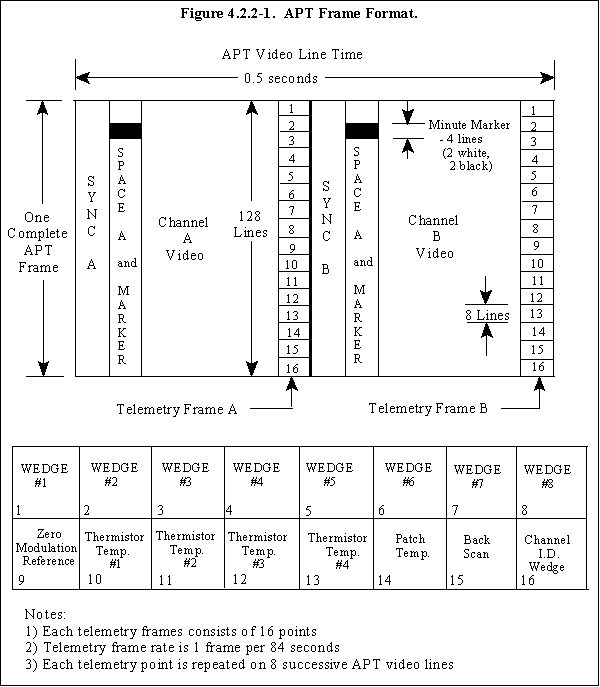
\includegraphics[height=0.5\paperwidth]{images/NOAA_APT_Frame_Format.png}
        \end{column}
    \end{columns}
\end{frame}
\begin{frame}
    \begin{center}
    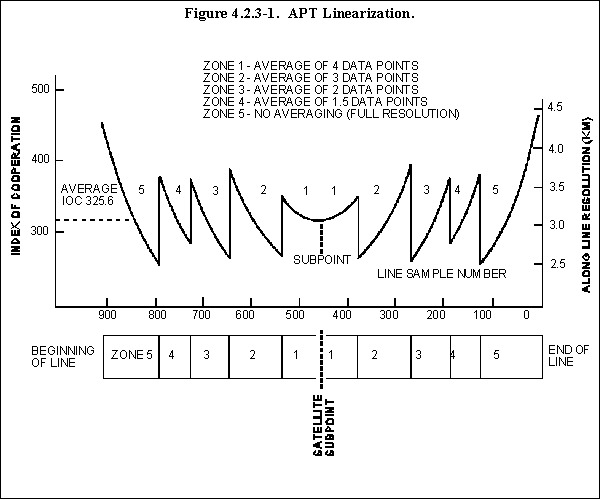
\includegraphics[width=0.75\paperwidth,height=1.0\paperheight,keepaspectratio]{images/apt-freq.jpg}
    \end{center}
\end{frame}
\subsection{Decoding Meteor LRPT}
\begin{frame}
    Meteor is digital (compared to NOAA analog)
\end{frame}
\begin{frame}
    Show QAM signal
\end{frame}
\begin{frame}
    Image of waterfall comparison
\end{frame}
\begin{frame}
    Decode digital signal, then process to image
\end{frame}
\section[Images]{Previously Captured Images}
\frame{\sectionpage}
{\usebackgroundtemplate{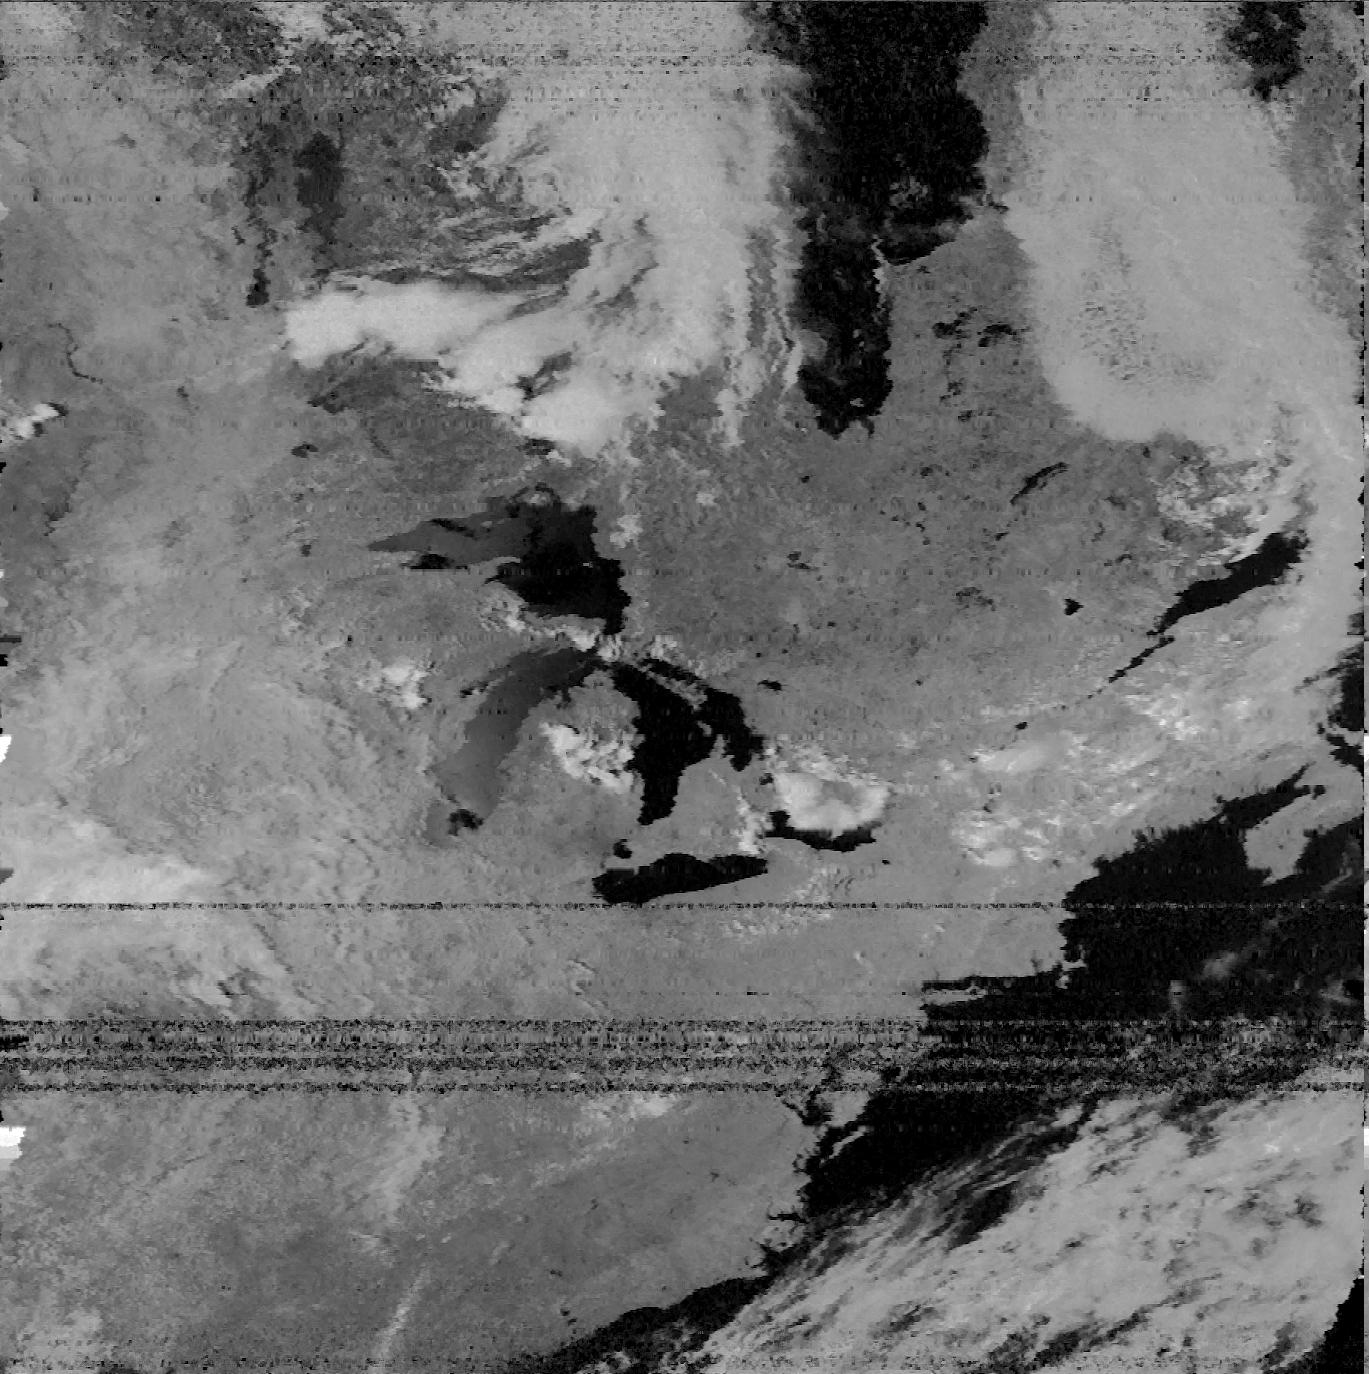
\includegraphics[height=1.0\paperheight,width=1.0\paperwidth,keepaspectratio]{images/apt-nomap.png}}
\begin{frame}[plain]
\end{frame}}
{\usebackgroundtemplate{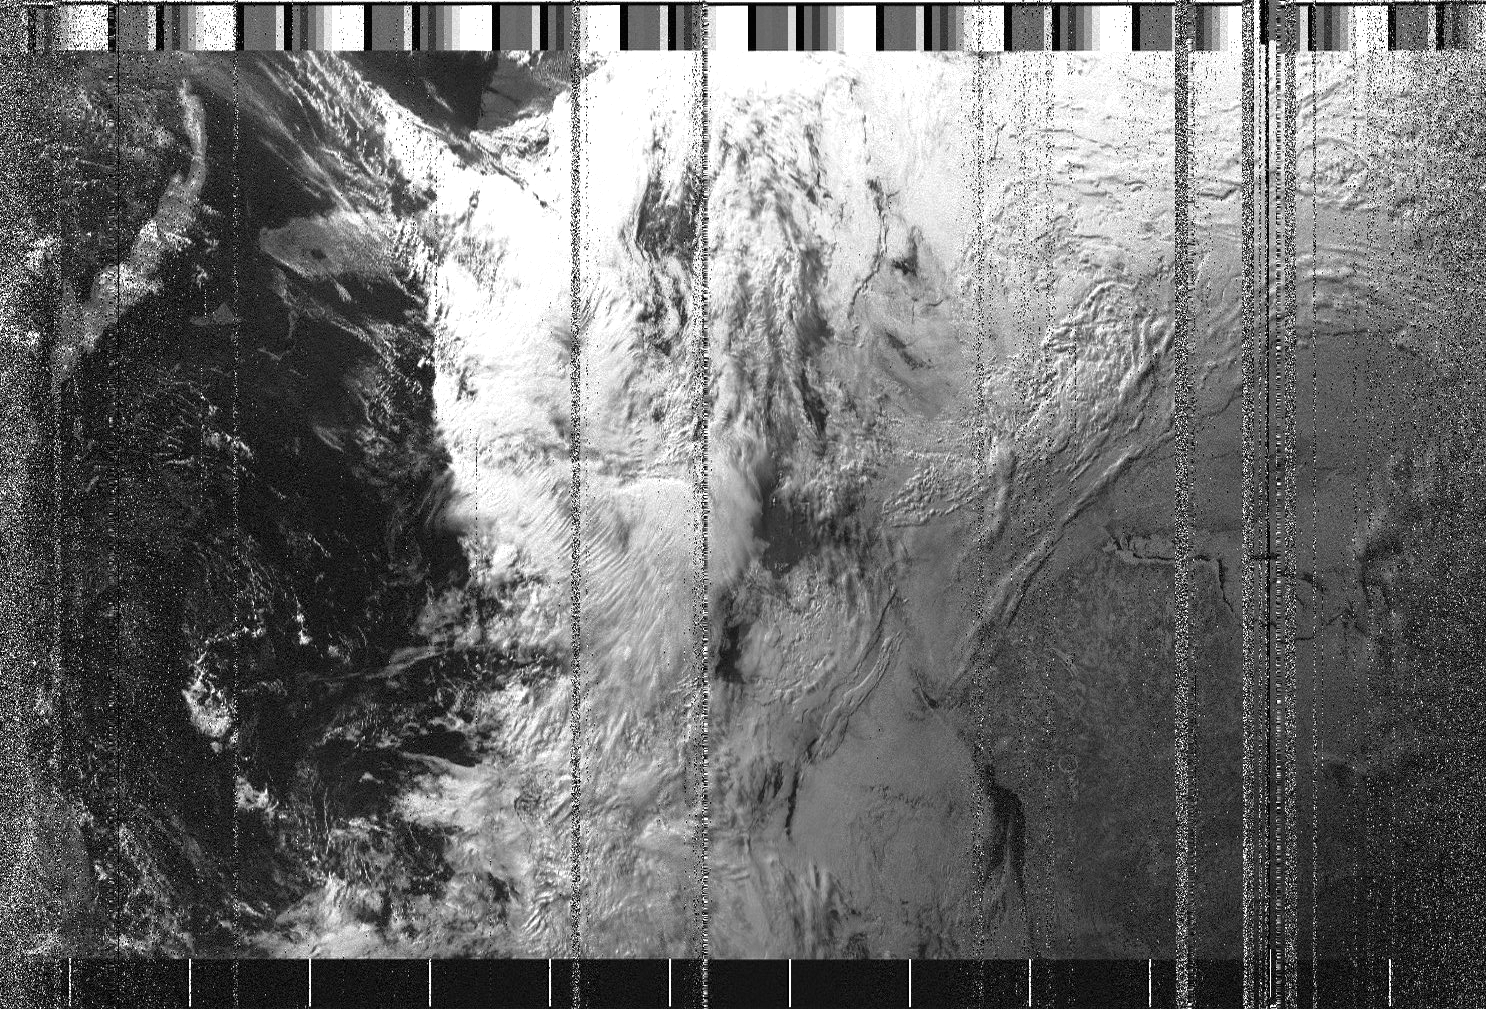
\includegraphics[height=1.0\paperheight,keepaspectratio]{images/noaa19-jan17.png}}
\begin{frame}[plain]
\end{frame}}
{\usebackgroundtemplate{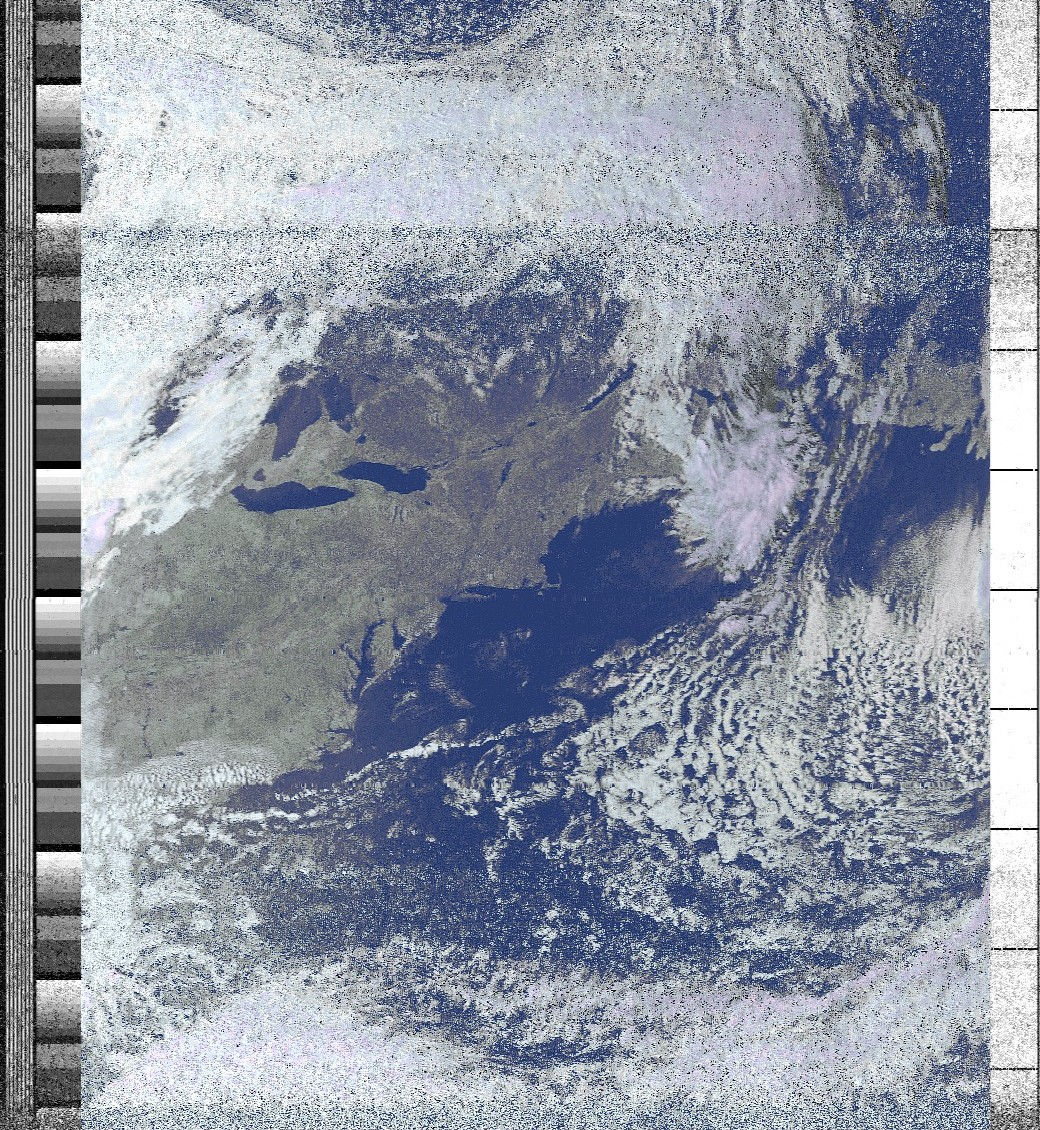
\includegraphics[height=1.0\paperheight,keepaspectratio]{images/noaa-19-03-10-2017-1941-hvct.jpg}}
\begin{frame}[plain]
\end{frame}}
{\usebackgroundtemplate{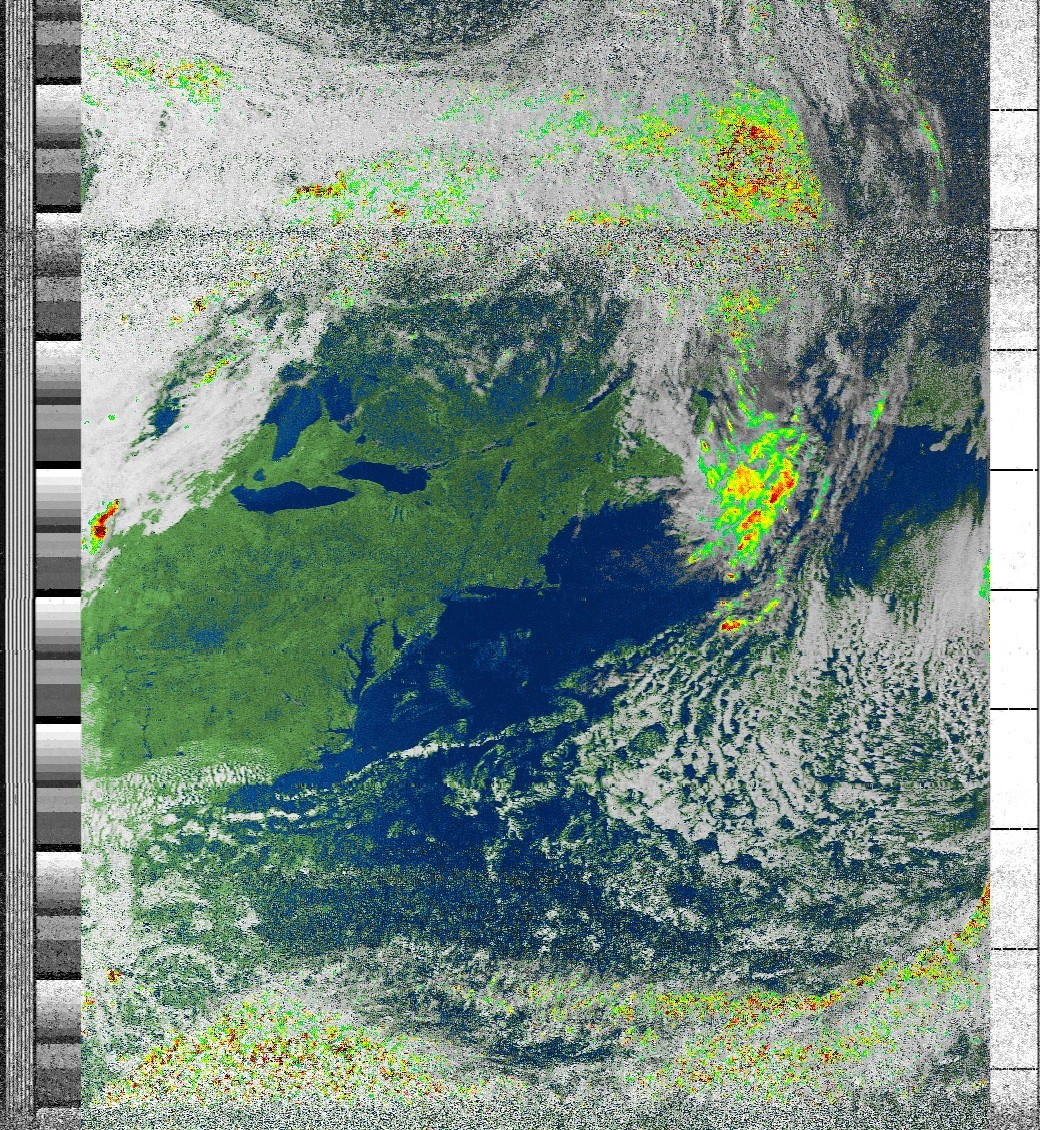
\includegraphics[height=1.0\paperheight,keepaspectratio]{images/noaa-19-03-10-2017-1941-msa-precip.jpg}}
\begin{frame}[plain]
\end{frame}}
{\usebackgroundtemplate{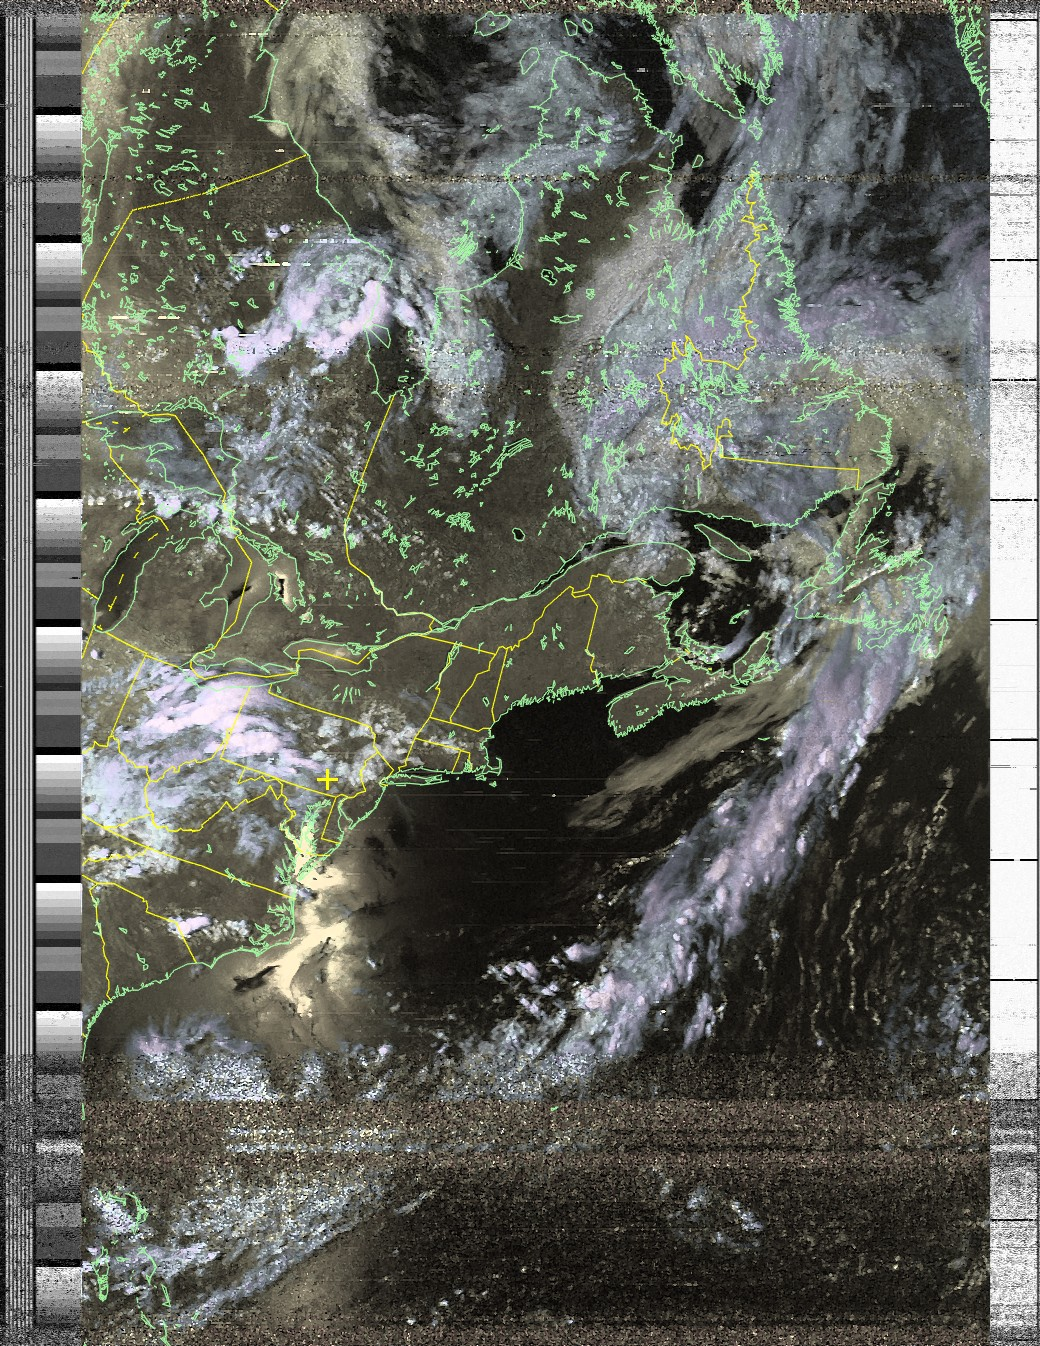
\includegraphics[height=1.0\paperheight,keepaspectratio]{images/noaa-19-10-08-2018-2007-hvc.jpg}}
\begin{frame}[plain]
\end{frame}}
{\usebackgroundtemplate{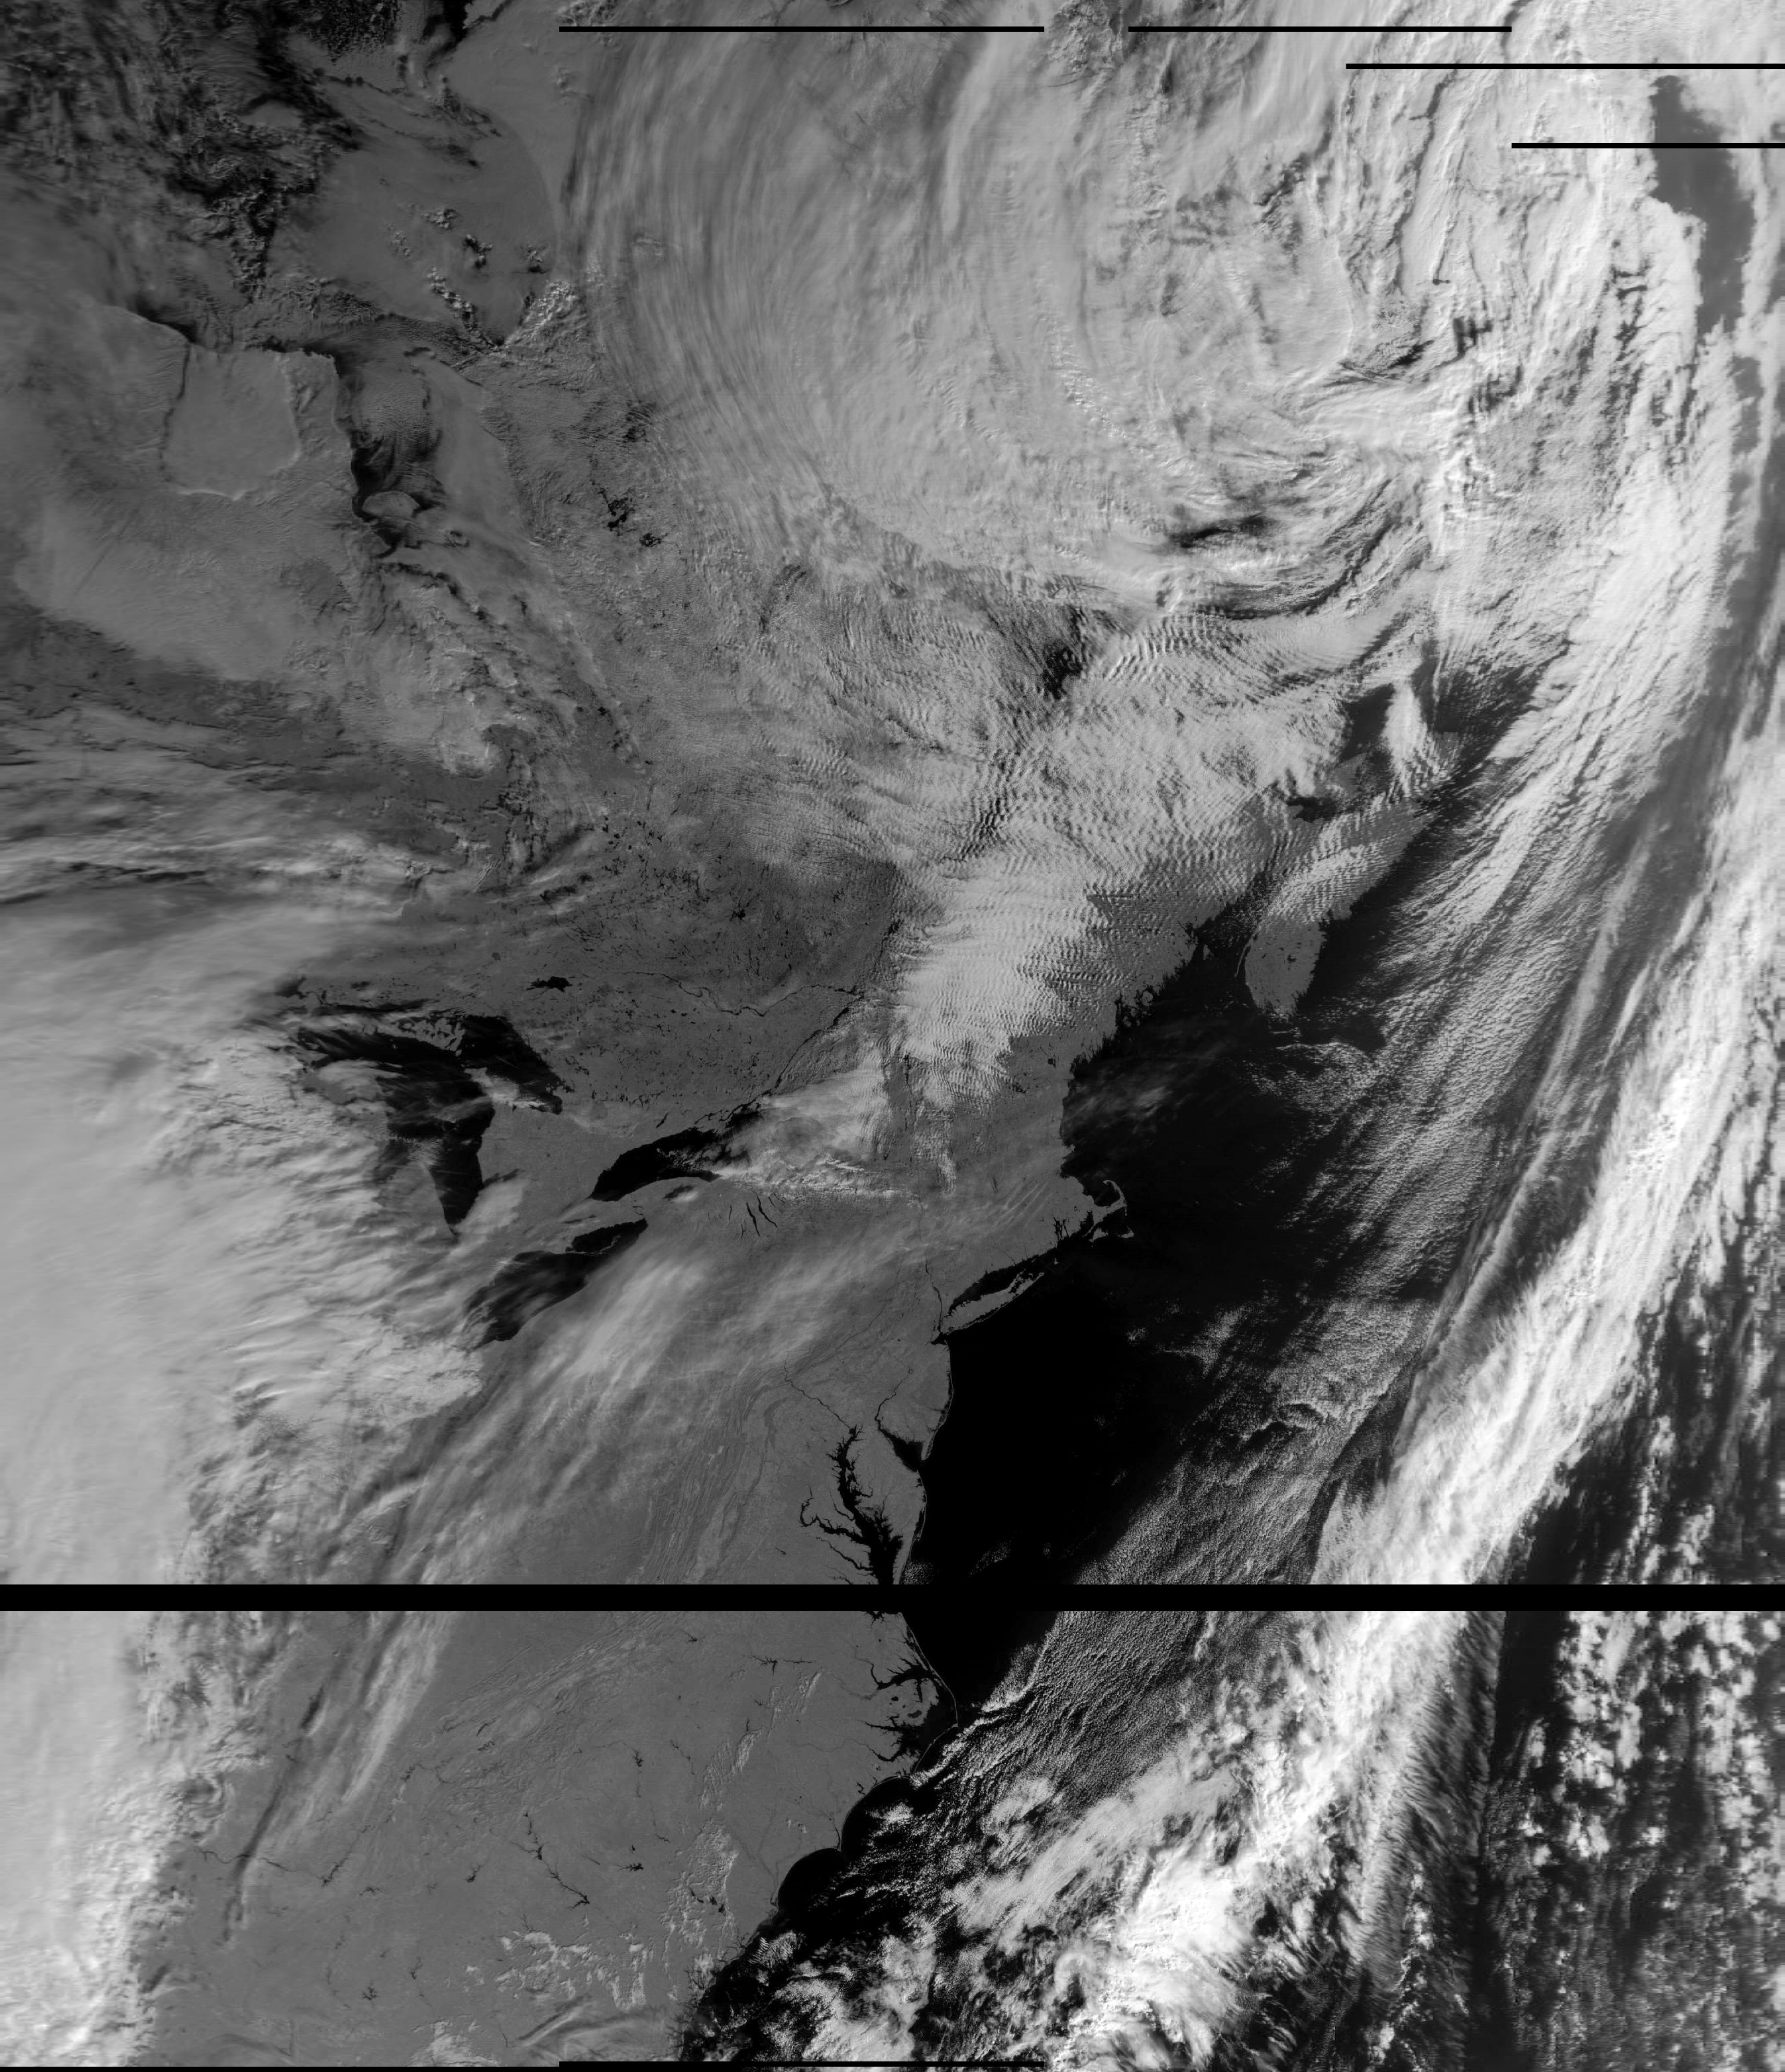
\includegraphics[height=1.0\paperheight,keepaspectratio]{images/meteorm2-full.png}}
\begin{frame}[plain]
\end{frame}}
{\usebackgroundtemplate{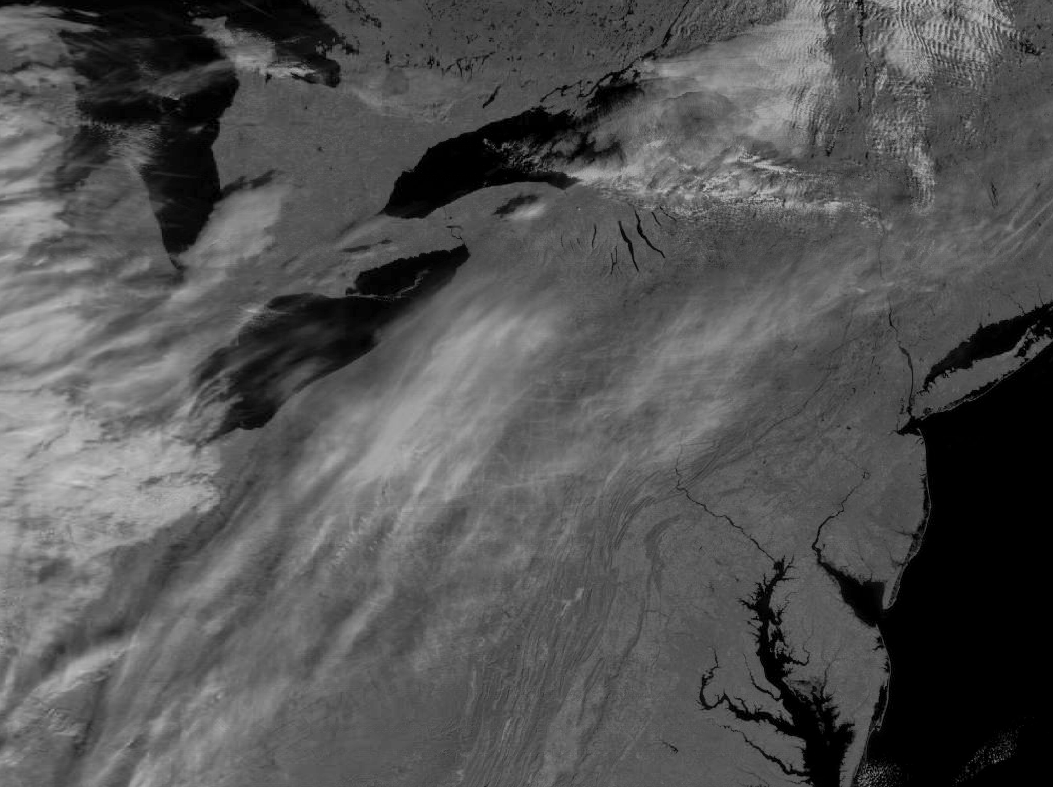
\includegraphics[height=1.0\paperheight,keepaspectratio]{images/meteorm2-crop.png}}
\begin{frame}[plain]
\end{frame}}
{\usebackgroundtemplate{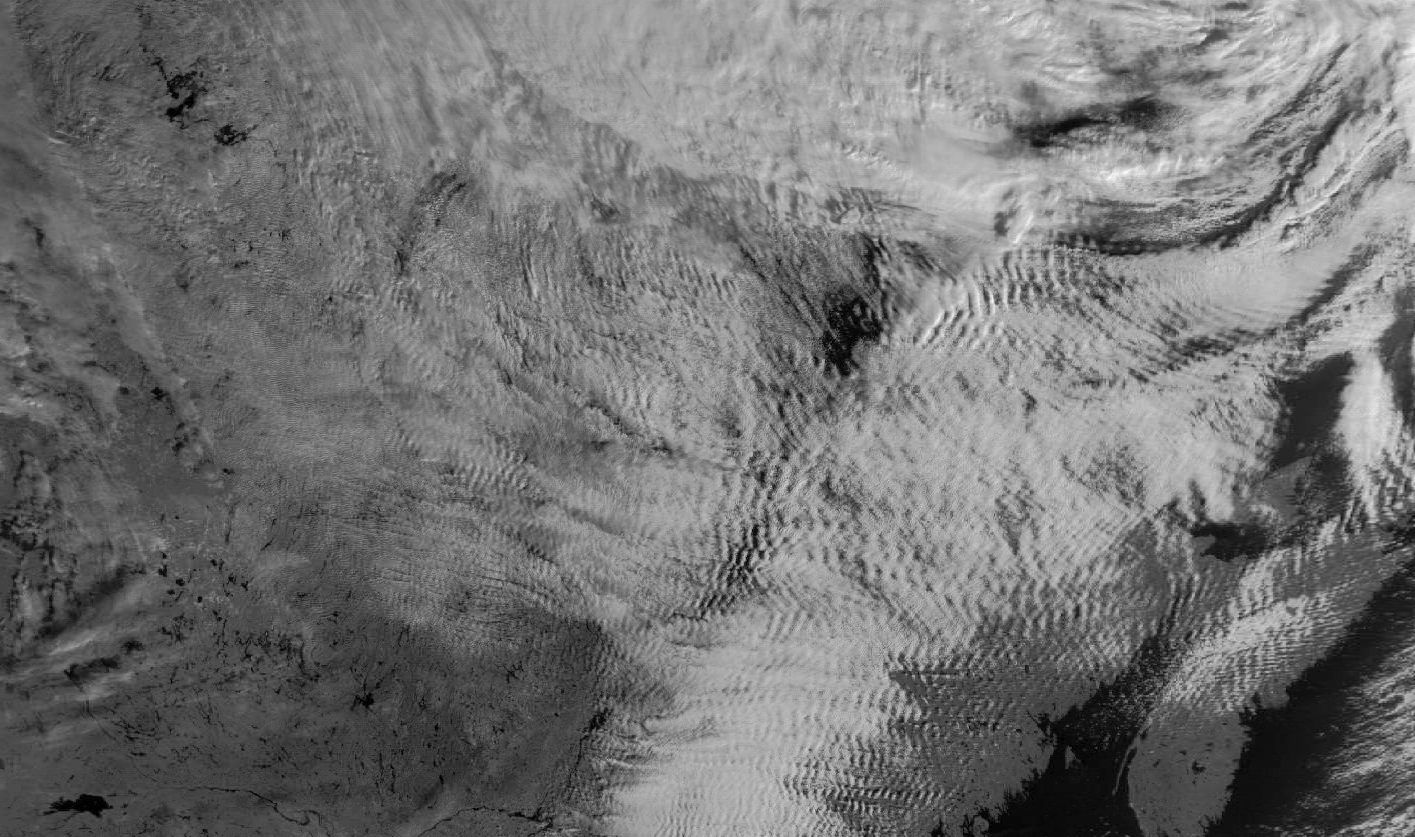
\includegraphics[height=1.0\paperheight,keepaspectratio]{images/meteorm2-ca-clouds.png}}
\begin{frame}[plain]
\end{frame}}


\section{Questions}
\frame{\sectionpage}
\end{document}

% vim: set ts=4 sw=4:
